 %GPL V3 by Mathias Hablützel, feel free to improve this template
 \documentclass[a4paper,10pt]{article}
 
 % Use UTF8 since the laptop is configured so and use ngerman for word breaking.
 % If you encounter an encoding problem, remove the line with utf8.
 \usepackage[utf8]{inputenc}
 \usepackage[ngerman]{babel}
 \usepackage[pdftex]{graphicx}
 
 % TikZ für schöne Grafiken und so.
 \usepackage{tikz}
 \usetikzlibrary{positioning,calc,fadings,decorations.pathreplacing,arrows}
 \usepackage{pgfplots}

% \usepackage{hyperref}
 \usepackage{colortbl}
 \usepackage{tabularx}
 \usepackage{color}
 \usepackage{amsfonts}
 \usepackage{amsmath}
 \usepackage{gensymb}
 \usepackage{listings}
 \usepackage{multirow}
 \usepackage{fancyhdr}
 \usepackage{multicol}
 \usepackage{wrapfig}
 \usepackage{pdfpages}
 \usepackage[colorlinks=true,
  linkcolor=black,
  citecolor=black,
  filecolor=black,
  pagecolor=black,
  urlcolor=black,
  bookmarks=true,
  bookmarksopen=true,
  bookmarksopenlevel=3,
  plainpages=false,
  pdfpagelabels=true]{hyperref}

% Hack for german umlaute
\lstset{
  literate={ö}{{\"o}}1
           {ä}{{\"a}}1
           {ü}{{\"u}}1
}

% define colors
 \definecolor{hellgrau}{rgb}{0.8,0.8,0.8}

  % http://stackoverflow.com/questions/741985/latex-source-code-listing-like-in-professional-books
  \usepackage{listings}
  \usepackage{courier}
 \lstset{
         basicstyle=\footnotesize\ttfamily, % Standardschrift
         numbers=left,               % Ort der Zeilennummern
         numberstyle=\tiny,          % Stil der Zeilennummern
         stepnumber=1,               % Abstand zwischen den Zeilennummern
         numbersep=5pt,              % Abstand der Nummern zum Text
         tabsize=2,                  % Groesse von Tabs
         extendedchars=true,         %
         breaklines=true,            % Zeilen werden Umgebrochen
         keywordstyle=\color{red},
    		frame=b,         
 %        keywordstyle=[1]\textbf,    % Stil der Keywords
 %        keywordstyle=[2]\textbf,    %
 %        keywordstyle=[3]\textbf,    %
 %        keywordstyle=[4]\textbf,   \sqrt{\sqrt{}} %
         stringstyle=\color{white}\ttfamily, % Farbe der String
         showspaces=false,           % Leerzeichen anzeigen ?
         showtabs=false,             % Tabs anzeigen ?
         xleftmargin=17pt,
         framexleftmargin=17pt,
         framexrightmargin=5pt,
         framexbottommargin=4pt,
         %backgroundcolor=\color{lightgray},
         showstringspaces=false      % Leerzeichen in Strings anzeigen ?        
 }
 \lstloadlanguages{% Check Dokumentation for further languages ...
         %[Visual]Basic
         %Pascal
         %C
         %C++
         %XML
         %HTML
         Java
 }
    %\DeclareCaptionFont{blue}{\color{blue}} 

  %\captionsetup[lstlisting]{singlelinecheck=false, labelfont={blue}, textfont={blue}}
  \usepackage{caption}
\DeclareCaptionFont{white}{\color{white}}
\DeclareCaptionFormat{listing}{\colorbox[cmyk]{0.43, 0.35, 0.35,0.01}{\parbox{\textwidth}{\hspace{15pt}#1#2#3}}}
\captionsetup[lstlisting]{format=listing,labelfont=white,textfont=white, singlelinecheck=false, margin=0pt, font={bf,footnotesize}}


 % I set here a different sidemargin because the original margin looks not so
 % good for normal documents. Additionally I have to enlarge the textwidth.
 \setlength{\oddsidemargin}{0cm}
 \setlength{\evensidemargin}{0cm}
 \addtolength{\textwidth}{4cm}
\newcolumntype{C}[1]{>{\centering\arraybackslash}m{#1}} 

\begin{document} 
 % Here I use the up-to-date font encoding T1 and the font familly Computer Modern
 % Sans Serif (since I don't like the standard font) medium and normal (non-italic or so).
\usefont{T1}{cmss}{m}{n}

\pagestyle{fancy} %eigener Seitenstil
\fancyhf{} %alle Kopf- und Fußzeilenfelder bereinigen
\fancyhead[C]{LakeRouting - Optimale Wegfindung anhand von Wettermodellen} %zentrierte Kopfzeile
\renewcommand{\headrulewidth}{0.4pt} 
\fancyfoot[C]{\thepage}

\title{
 \begin{flushleft}
  \vspace*{-3cm}
  
\includegraphics[keepaspectratio,width=7cm]{img/de-zhaw-cmyk}
 \end{flushleft}
 \vspace*{4cm}
 LakeRouting - Optimale Wegfindung anhand von Wettermodellen
}

\date{\today}
\author{Fevzi Yükseldi (yuksefev@students.zhaw.ch)\\
 Mathias Hablützel (hablumat@students.zhaw.ch)\\
 \\
 Dr. Rudolf M. Füchslin (furu@zhaw.ch)\\
 Prof. Dr. Peter T. Früh (frup@zhaw.ch)\\
 Jacques Ambühl (jacques.ambuehl@meteoschweiz.ch)
}
 
\maketitle

\thispagestyle{empty}
\newpage
\thispagestyle{empty}

\part*{Management Summary}

\vspace*{2cm}
\setlength{\columnsep}{2cm}
\begin{multicols}{2}

\textbf{\textsc{Deutsch}}
\vspace{1cm}\\

\columnbreak

\textbf{\textsc{English}}
\vspace{1cm}\\

\end{multicols}
\newpage

\cleardoublepage
\begingroup
\pagestyle{empty}
\setcounter{tocdepth}{2}
\tableofcontents
\clearpage
\endgroup
       
\newpage

\setcounter{page}{1} 
\part{Einleitung}
\section{Ausgangslage}
Zu den klassischen Methoden der mathematischen Entscheidungsvorbereitung gehört
die Dynamische Programmierung (DP). Sie ermöglicht die optimale Gestaltung
einer Kette sequentieller Entscheidungen aufgrund wettbewerbsrelevanter
Randbedingungen (physikalischer oder ökonomischer Natur).

Richard Bellman hat den Begriff 1940 eingeführt. Der Wortteil dynamisch
bezieht sich auf eine ursprüngliche Zeitvariabilität in Kombination des Lösens
eines Problems -- von Bellman als Programm bezeichnet -- und soll den
Gegensatz zum linearen Lösen von Problemen verdeutlichen.

Sehr viele bekannte Probleme können effizient mittels dynamischen
Programmierens gelöst werden, so zum Beispiel das travelling salesmen problem,
das maximum subarray problem oder auch longest common subsequence problem, die
alle eine sehr hohe Bedeutung in der Informatik haben und jedem Informatiker
in der einen oder anderen Art bekannt sind.

So wollte auch die MeteoSchweiz mittels dieser Methode eine Problemstellung
in Java implementiert haben, die bereits von einem ihrer Mitarbeiter in
Mathematica entworfen wurde.

\section{Auftrag}
Die Bachelorarbeit ist eine Anwendung der dynamische Programmierung zur
Kursbestimmung eines Segelschiffs. Aufgrund der mit einem numerischen
Modell vorausgesagten Wetterentwicklung und in Anbetracht der Leistungskurve
(Polardiagramm) des Schiffes wird dessen optimale Route mittels dynamische
Programmierung berechnet. Ähnliche Methoden wurden beim Alinghi Team im Rahmen
des Americas Cup verwendet.

\subsection{Systemspezifikation}
Die Programmiersprache ist mit Java vorgegeben. Es sind keine weiteren
Einschränkung wie das verwenden eines bestimmten Frameworks, Librarys oder
eines bestimmten Betriebsystemes.

\subsection{Öffentlichkeitsarbeit, Auftritte}
Von der Seite der ZHAW ist die obligatorische Bachelorarbeits-Präsentation
gegeben und zählt als Bewertungsteil der Gesamtarbeit. Die MeteoSchweiz will
die Arbeit bei mindestens einem internen Vortrag präsentieren, weitere
Auftritte können mit den Autoren der Arbeit vereinbart werden.

\subsubsection{Weitere Verwendung der Arbeit}
Weitere Anwendungen der dynamischen Programmierung zum Thema ''energy
trading'' für erneuerbare Energiequellen sind denkbar und eine Übertragung der
Resultate der Bachelorarbeit in diesen Bereich werden von MeteoSchweiz
angestrebt.

\subsection{Terminologie}
\paragraph{Seemeile}ist eine in der Meteorologie gebräuchliche Längeneinheit,
die als Berechnungsgrundlage für die Navigation und das Angeben von Distanzen
dient. Sie entspricht der Länge einer Winkelminute eines Grosskreis und auf der
Erde beträgt diese Distanz 1852 m.

\paragraph{Winkelminute}ist der sechzigste Teil eines Winkelgrades, welches
wiederum der dreihundertsechzigste Teil einer Umdrehung ist. Somit wäre eine
Winkelminute \\ \( W=\frac{1 Grad}{60} = 0.0\overline{16}^\circ \)

\paragraph{Knoten}ist ein Geschwindigkeitsmass in der Meteorologie, das auf der
Längeneinheit Seemeile beruht. Somit ist ein Knoten 1852 m/h = 0.514 m/s.


\section{Weitere Informationen sowie Danksagung}
Für das gelingen dieser Arbeit haben viele Personen beigetragen, insbesondere
bei unseren beiden Betreuer Herr Dr. R. Füchslin und Herrn J. Ambühl möchten
wir uns für die grosse Geduld, ihre Hilfe und ihren ehrlichen Rückmeldungen
bedanken. Nicht selbstverständlich ist es, dass unser direktes Umfeld,
Mitstudenten, Freunde, Familie unsere Launen, Arbeitswut und teils lautstark
kund gemachten Frustrationen ertrugen, auch denen möchten wir an dieser Stelle
danken.

\subsection{Mathias dankt \dots}
Ich möchte an dieser Stelle allen Leuten von der NGAS-Crew und der ehemaligen
Forkbomb-Crew danken, die mir in ihrer Freizeit die Skills vermittelt haben,
die ich heute habe und bei dieser Arbeit einsetzen konnte. Zugleich möchte ich
den Entwickler aller von mir im Rahmen dieser Arbeit verwendeten Tools danken,
dass sie mir meine Arbeit so ungemein erleichtert haben.

Eine grosse Unterstützung waren und sind die Freunde Astrid, Daniela, Dario,
Juliane, Martina, Michael, Miriam, René und Tonnerre, die teils zu unmöglichen
Zeiten für mich da waren, mir zugehört, Mut gemacht haben und ohne die ich
nicht zu dem Mensch geworden wäre, der ich heute bin.

\subsection{Fevzi dankt \dots}

\newpage
\part{Vorgehen / Methoden}
\section{Dynamische Programmierung}
Der Begriff dynamische Programmierung wurde erstmals in den 1940er Jahren von
Richard Bellman benutzt und umfasst eine Reihe von Methoden mit dem Ziel,
Optimierungsprobleme zu lösen. 

Das Optimierungsproblem wird dann erfolgreich mit diesem Verfahren
gelöst, wenn sie in mehrere gleichartige Teilprobleme aufgeteilt werden
kann. Eine optimale Lösung setzt sich somit aus den optimalen Lösungen
der Teilproblemen zusammen, wobei die Randbedingungen der Teilproblemen
voneinander abhängen können.  Aus diesem Grund ist eine Strategie dann
optimal, wenn alle Unterstrategien optimal sind. Die Zwischenergebnisse
der Teilprobleme werden aber nicht rekursiv, sondern iterativ berechnet
und in einer Tabelle gespeichert, so dass, wenn sie wieder benötigt
werden, nicht nochmals berechnet werden müssen.

In unserer Anwendung ist das Ziel klar: Den Kurs des Segelschiffes zu
bestimmen indem man die zeitlich kürzeste Route vom Start- bis zum
Endpunkt berechnet. Dies erfolgt indem man die Strecke in Teilstrecken
aufteilt und die Dauer der Fahrt für diese Strecken berechnet. Danach
wird der Pfad mit der kleinsten Dauer bestimmt. Zu diesem Zweck werden
die Windvektoren auf der Wasseroberfläche und ihre Interaktion mit dem
Segelschiff in die Berechnung miteinbezogen. 

\subsection{Die ersten Schritte}
Betrachten wir nun ein Fahrzeug, welches sich auf der Erdoberfläche mit
einer konstanten Geschwindigkteit bewegt. Nehmen wir an, dass dieses
Fahrzeug von einem Anfangspunkt bis zu einem Ankunftspunkt reisen
möchte. Die Unterteilung, also die Zerstückelung der Strecke wird mit
der Aufspannung eines Gitternetzes zwischen diesen beiden Punkten
bereitgestellt.

Beginnend mit einer sehr einfachen Formulierung, die schrittweise verfeinert
werden soll, definiert man:

\( \Delta t_i\;,  i=0...m\), ist die benötigte Zeit von der \( (i-1)\)-ten
Spalte bis zur \(i\)-ten Spalte, wobei \(i=0\) der ersten Spalte entspricht,
wo sich der Anfangspunkt befindet und \(i=m\) der letzten Spalte entspricht,
wo sich der Ankunftspunkt befindet.

% TODO: Skizze vom Gitternetz mit delta_t und Spalten-Indizes hinzufügen

\( D_i\;,  i=0...m\), bis zu der \(i\)-ten Spalte benötigte Zeit.

Unser optimales Programm kann somit wie folgt definiert werden: "Minimierung
der Reisedauer \(D_m\) von der Spalte \(0\) bis \(m\)". 

\begin{equation}
\label{eq_dyn:1}
D_m = \min [\; \sum_{i=1}^m \Delta t_i\;]
 \end{equation}

Wenn wir eine Zwischenstufe \(I\) berechnen lassen, erhalten wir die
folgende, umgeschriebene Formel:

\begin{equation}
\label{eq_dyn:2}
D_I = \overset{I}{\underset{i=1}{\min}} [\; \Delta t_I + \sum_{i=1}^{I-1}
\Delta t_i\;] = \overset{I}{\min} [\; \Delta t_I +
\overset{I-1}{\underset{i=1}{\min}} [\; \sum_{i=1}^{I-1} \Delta t_i\;]\;] =
\overset{I}{\min} [\; \Delta t_I + D_{I-1} \;]
\end{equation}

Somit liefert die Gleichsetzung der ersten und letzten Ausdrücke eine rekursive
Formulierung des Problems. Desweiteren muss ein Anfangswert angegeben werden,
vorausgesetzt \(D_0  = D_{i=0} =\) Abfahrtszeit ist, so dass gilt:
 
 \begin{equation}
\label{eq_dyn:3}
D_I =  \overset{I}{\min} [\; \Delta t_I + D_{I-1} \;];\;\;\;\;\;\; D_0: Abfahrtszeit.
 \end{equation}
 
Diese Ableitung ergibt sich aus einer Optimierungsprinzip, dass eine
Strategie nur dann optimal ist, wenn alle ihre Unterstrategien optimal
sind. Und somit birgt eine solche pauschale Formulierung den
Entscheidungsprozess. 
 
Folglich gibt es zwei Entscheidungsverfahren:

\begin{itemize}
\item Bei jedem Knoten j in der Spalte I-1 soll eine Abfrage durchgeführt
werden, zu welchem Knoten k in der nächsten Spalte I das Segelschiff segeln
soll.
\item Bei jedem Knoten k in der Spalte I soll eine Abfrage durchgeführt werden,
von welchem Knoten j in der vorherigen Spalte I-1 das Segelschiff gesegelt
haben soll.
\end{itemize}

Die Einführung in die letzte Bedingung im vorherigen Ausdruck für \(D_I\)
ergibt (mit Standard-Typografie \{i,j\}  für die Darstellung von Knoten in der
Graphentheorie) wobei $n$ die Anzahl Knoten im Grafen auf jede Seite vom
Startpunkt als Mittelpunkt betrachtet ist:

\begin{equation}
\label{eq_dyn:4}
D_{(I,k)} = \overset{j=n}{\underset{j=-n}{\min}} [\; \Delta t_{\{I-1,j\}}^{\{I,k\}} + D_{(I-1.j)} \;];\;\;\;\;\;\; D_0: Abfahrtszeit.
\end{equation}

Der Knoten $j^*$ gehört zur Spalte $I-1$ und genügt dem oben geforderten
Minimum und wird somit als Lösung verwendet für den Knoten $k$ in Spalte $I$.

\begin{equation}
\label{eq_dyn:5}
D_{(I,k)} \to j^* \in Spalte\; I-1
\end{equation}
 
Es ist ersichtlich, dass der Ausdruck \(D\) - für die Dauer - auch sehr leicht
für Decision (dt. Entscheidung) gehandelt werden kann. Mit dieser Annahme,
beinhaltet der Ausdruck \(D_I\) in der Formel \eqref{eq_dyn:3} alle gewählten
Entscheidungen der Spalte I, und dies für jeden Knoten k einzeln in dieser
Spalte.

\begin{equation}
\label{eq_dyn:6}
D_I \to \{\;j_{-n}^*\; ... \;j_{k}^* \;...\; j_{n}^*\;\} \subset Spalte\; I-1
\end{equation}

Die Anzahl der Schritte vom Anfangspunkt bis zum Ankunftspunkt ist als \(m\)
und die Anzahl der Zeilen (Optionen) als n definiert, welche auch später näher
erläutert werden.
 
Eine weitere Verfeinerung muss eingeführt werden. Nehmen wir an, wir hätten ein
Knoten mit dem Index \{i,-n\} ausgewählt. Somit ist es laut unserem Algorithmus
möglich, dass der Vorgänger dieser Knotens den Index \{i-1,+n\} haben kann, was
einer seitlichen Kreuzung entspricht und eher unwahrscheinlich ist.

Deshalb braucht es einen Steuermechanismus, der die Anzahl der möglichen
Adressierungen von einem Knoten \{i, k\} mit den Knoten der vorherigen Spalte
\{i-1, k\} begrenzt. Dies wird mit dem Spread-Parameter erreicht und sieht dann
wie folgt aus:

\begin{equation}
\label{eq_dyn:7}
D_{I,k} \to j^*\; mit\; |\;j^*\;-\;k\;| \;\le\; Spread;\; j^*\; \in Spalte\; I-1
\end{equation}
 
Somit werden nur die Knoten in der Spalte \(i\) als Nachbarn für die Knoten in
der Spalte \(i-1\) gelten, welche auch diese Bedingung erfüllen. Die restlichen
Knoten der Spalte \(i\), die diese Bedingung nicht erfüllen, werden einfach bei
der Auswahl nicht berücksichtigt.

Der Spread-Parameter wird uns später auch einen weiteren Vorteil bringen. Er
wird uns helfen die Problematik mit der Küste zu bewältigen, so dass
unsere Route nicht das Gewässer verlässt.

\newcommand\pgfmathsinandcos[3]{%
  \pgfmathsetmacro#1{sin(#3)}%
  \pgfmathsetmacro#2{cos(#3)}%
}

\newcommand\LongitudePlane[3][current plane]{%
  \pgfmathsinandcos\sinEl\cosEl{#2} % elevation
  \pgfmathsinandcos\sint\cost{#3} % azimuth
  \tikzset{#1/.estyle={cm={\cost,\sint*\sinEl,0,\cosEl,(0,0)}}}
}

\newcommand\LatitudePlane[3][current plane]{%
  \pgfmathsinandcos\sinEl\cosEl{#2} % elevation
  \pgfmathsinandcos\sint\cost{#3} % latitude
  \pgfmathsetmacro\yshift{\cosEl*\sint}
  \tikzset{#1/.estyle={cm={\cost,0,0,\cost*\sinEl,(0,\yshift)}}} %
}

\newcommand\DrawLongitudeCircle[2][1]{
  \LongitudePlane{\angEl}{#2}
  \tikzset{current plane/.prefix style={scale=#1}}
   % angle of "visibility"
  \pgfmathsetmacro\angVis{atan(sin(#2)*cos(\angEl)/sin(\angEl))} %
  \draw[current plane,thin,black] (\angVis:1) arc (\angVis:\angVis+180:1);
  \draw[current plane,thin,dashed] (\angVis-180:1) arc (\angVis-180:\angVis:1);
}%this is fake: for drawing the grid


\newcommand\DrawLongitudeCirclered[2][1]{
  \LongitudePlane{\angEl}{#2}
  \tikzset{current plane/.prefix style={scale=#1}}
   % angle of "visibility"
  \pgfmathsetmacro\angVis{atan(sin(#2)*cos(\angEl)/sin(\angEl))} %
  \draw[current plane,red,thick] (150:1) arc (150:180:1);
  %\draw[current plane,dashed] (-50:1) arc (-50:-35:1);
}%for drawing the grid


\newcommand\DLongredd[2][1]{
  \LongitudePlane{\angEl}{#2}
  \tikzset{current plane/.prefix style={scale=#1}}
   % angle of "visibility"
  \pgfmathsetmacro\angVis{atan(sin(#2)*cos(\angEl)/sin(\angEl))} %
  \draw[current plane,black,dashed, ultra thick] (150:1) arc (150:180:1);
}


\newcommand\DLatred[2][1]{
  \LatitudePlane{\angEl}{#2}
  \tikzset{current plane/.prefix style={scale=#1}}
  \pgfmathsetmacro\sinVis{sin(#2)/cos(#2)*sin(\angEl)/cos(\angEl)}
  % angle of "visibility"
  \pgfmathsetmacro\angVis{asin(min(1,max(\sinVis,-1)))}
  \draw[current plane,dashed,black,ultra thick] (-50:1) arc (-50:-35:1);
}


\newcommand\fillred[2][1]{
  \LongitudePlane{\angEl}{#2}
  \tikzset{current plane/.prefix style={scale=#1}}
   % angle of "visibility"
  \pgfmathsetmacro\angVis{atan(sin(#2)*cos(\angEl)/sin(\angEl))} %
  \draw[current plane,red,thin] (\angVis:1) arc (\angVis:\angVis+180:1);
}

\newcommand\DrawLatitudeCircle[2][1]{
  \LatitudePlane{\angEl}{#2}
  \tikzset{current plane/.prefix style={scale=#1}}
  \pgfmathsetmacro\sinVis{sin(#2)/cos(#2)*sin(\angEl)/cos(\angEl)}
  % angle of "visibility"
  \pgfmathsetmacro\angVis{asin(min(1,max(\sinVis,-1)))}
  \draw[current plane,thin,black] (\angVis:1) arc (\angVis:-\angVis-180:1);
  \draw[current plane,thin,dashed] (180-\angVis:1) arc (180-\angVis:\angVis:1);
}%Defining functions to draw limited latitude circles (for the red mesh)


\newcommand\DrawLatitudeCirclered[2][1]{
  \LatitudePlane{\angEl}{#2}
  \tikzset{current plane/.prefix style={scale=#1}}
  \pgfmathsetmacro\sinVis{sin(#2)/cos(#2)*sin(\angEl)/cos(\angEl)}
  % angle of "visibility"
  \pgfmathsetmacro\angVis{asin(min(1,max(\sinVis,-1)))}
  %\draw[current plane,red,thick] (-\angVis-50:1) arc (-\angVis-50:-\angVis-20:1);
\draw[current plane,red,thick] (-50:1) arc (-50:-35:1);
}


\tikzset{
  >=latex,
  inner sep=0pt,
  outer sep=2pt,
  mark coordinate/.style={inner sep=0pt,outer sep=0pt,minimum size=3pt, fill=black,circle}
}


\section{Aufgabe 1 - Orthodromie}
\subsection{Aufgabenstellung}
\begin{itemize}
  \item Erstellung eines Entscheidungsnetzes auf der Erdkugel
  \item Berechnung einer Orthodromie (Distanz in Meilen zwischen zwei Punkten auf der Erdkugel)
  \item Erstellung der Koordinatendatei eines Sees (in Koordinaten)
\end{itemize}

\subsection{Analyse der Problemstellung}
Auf einer Kugel soll zwischen zwei Punkten die kürzeste Route bzw. die kürzeste Verbindung gewählt werden. Dies wird durch das Vektorprodukt der beiden Vektoren vom Kugelursprung zu den beiden Punkten $A$ und $B$ einfach berechnet:

\begin{tikzpicture}[scale=1,every node/.style={minimum size=1cm}]
	%% some definitions
	
	\def\R{4} % sphere radius
	
	\def\angEl{25} % elevation angle
	\def\angAz{-100} % azimuth angle
	\def\angPhiOne{-50} % longitude of point P
	\def\angPhiTwo{-15} % longitude of point Q
	\def\angBeta{30} % latitude of point P and Q
	
	%% working planes
	
	\pgfmathsetmacro\H{\R*cos(\angEl)} % distance to north pole
	\LongitudePlane[xzplane]{\angEl}{\angAz}
	\LongitudePlane[pzplane]{\angEl}{\angPhiOne}
	\LongitudePlane[qzplane]{\angEl}{\angPhiTwo}
	\LatitudePlane[equator]{\angEl}{0}
	\fill[ball color=white!10] (0,0) circle (\R); % 3D lighting effect
	\coordinate (O) at (0,0);
	\coordinate[mark coordinate] (N) at (0,\H);
	\coordinate[mark coordinate] (S) at (0,-\H);
	
    \DrawLongitudeCircle[\R]{\angPhiOne} % pzplane
    \DrawLongitudeCircle[\R]{\angPhiTwo} % qzplane
    \DrawLatitudeCircle[\R]{\angBeta}
    \DrawLatitudeCircle[\R]{0} % equator
	%labelling north and south
	\node[above=8pt] at (N) {$\mathbf{N}$};
	\node[below=8pt] at (S) {$\mathbf{S}$};
        \draw[-,dashed, thick] (N) -- (S);	
    	
\end{tikzpicture}


% Author: Mathias Hablützel

\section{Erfassung Schiffsgeschwindigkeiten}

\subsection{Problemanalyse}
\subsubsection{Windangriffswinkel und Windgeschwindigkeit}

\begin{wrapfigure}{r}{6cm} 
\centering
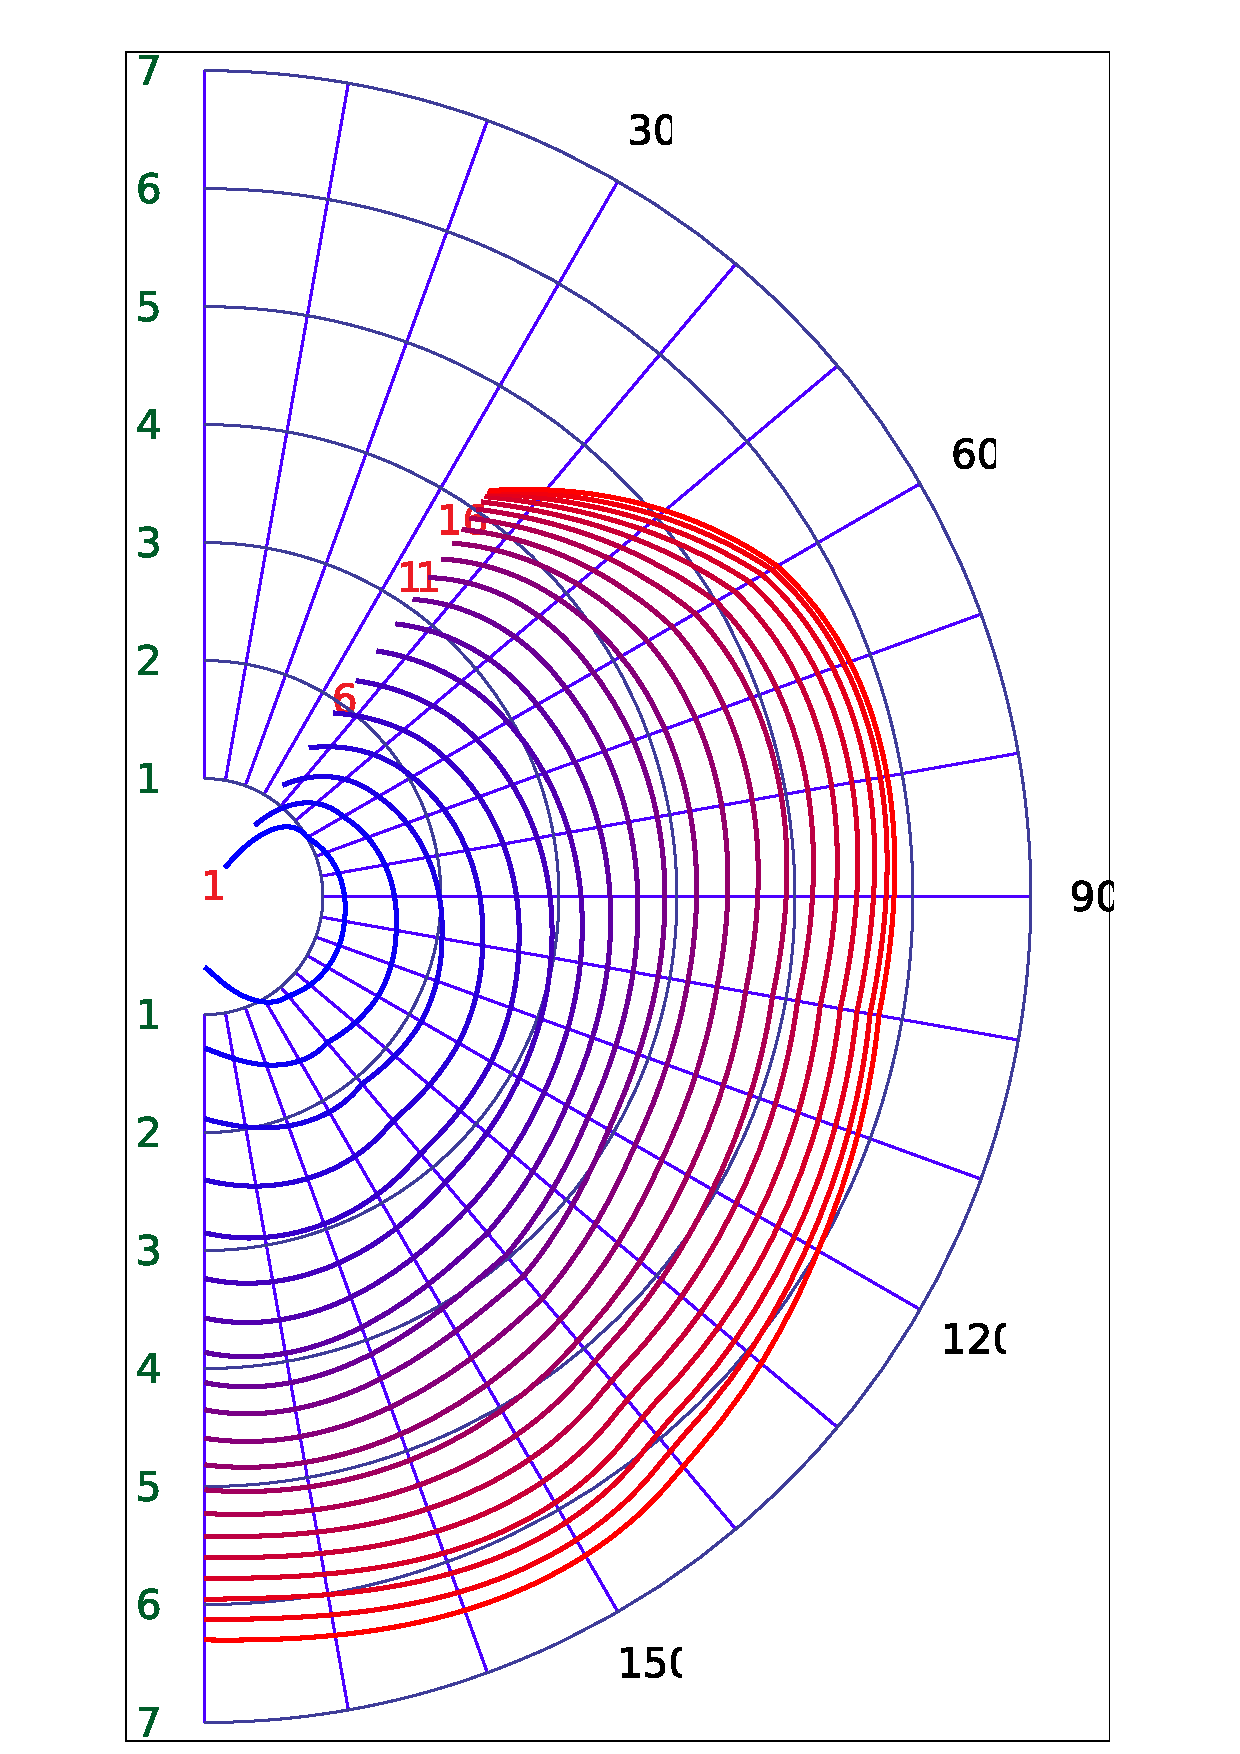
\includegraphics[width=6cm]{img/polardiagramm}
\caption{Polardiagramm eines Bootes, grün Windstärke in Knoten, rot
Geschwindigkeit in Knoten, schwarz Windangriffswinkel}
\label{polardiagram}
\end{wrapfigure}

Je nach Einfallswinkel des Windes variert die Schiffsgeschwindigkeit
stark. Bei frontal kommenden Wind fährt das Schiff gar nicht mehr
vorwärts und muss für diesen Umstand aufkreuzen, das heisst einen
Zickzack-Kurs fahren. Deshalb muss für jedes Schiff empirisch der
minimale Einfallswinkels vom Bug aus ermittelt werden, somit ist der
steilste Winkel bekannt.

Die Schiffsgeschwindigkeit variert aufgrund der physischen Eigenschaften
von Segel, Rumpf und Aerodynamik. Entgegen Intuition ist Wind von
Achtern nicht der schnellste, sondern bei sogenannt halben Wind (meist
zwischen 80\degree und 105\degree). Da sich diese Daten nicht nur bei
unterschiedlichen Einfallswinkel verändern, sondern auch bei
unterschiedlichen Windgeschwindigkeiten, empfiehlt es sich ein
sogenanntes Polardiagramm zu erstellen, dass die unterschiedliche
Fahrtgeschwindigkeiten in Bezug zu Einfallswinkel und
Windgeschwindigkeit darstellt.

Da aber der Datensatz nicht durchgehend ist, muss zwischen den bekannten
und ermittelten Punkten interpoliert werden.

\subsubsection{Interpolationsverfahren}
Um diese Daten zu interpolieren eignet sich die bilineare Interpolation
am besten, da sie sehr einfach zu implementieren ist, über eine für
unsere Zwecke genügend hohe Genauigkeit verfügt, in linearer Zeit
rechnet und nur aus Multiplikationen sowie Additionen besteht, was
aufgrund von den heutigen CPU-Befehlen nur noch wenigen Taktzyklen
braucht und somit zu einer sehr hohen Ausführgeschwindigkeit führt.

Andere Interpolationsmethoden wie qubische Interpolation,
Spline-Interpolation oder polynomielle Interpolation sind entweder zu
ressourcen konsumierend, langsam oder sogar instabil. Daher wurde diese
nicht in Betracht gezogen. Ausserdem verwendet dieses Verfahren nur die
unmittelbaren Nachbarwerte und kommt damit mit weniger Informationen
zurecht.

\subsection{Implementation}
\subsubsection{Eingabedaten-Parser}
Die Schiffsdaten sind als CSV\footnote{Comma Separated Values}-Datei
gegeben und werden von einem selbst\-geschriebenen Parser in ein
passendes Klassen-Konstrukt geladen. Die Schwierigkeit bestand darin,
dass die Daten nicht-dekoriert sind und daher nur durch ihre Position
von anderen Typen zu unterscheiden sind. Das bedeutet allerdings auch,
dass der Parser sich auf diese Datenstruktur verlässt und keine
Abweichungen duldet und sonst abstürzt.

Dieses Problem ist allerdings vertretbar, da die Datenstruktur
vorgegeben ist und der Parser daran angepasst wurde.

\subsubsection{Verarbeitungsklasse}
Die Klasse \texttt{BoatSpeedDiagram.java\footnote{Im Package 
ch.zhaw.lakerouting.interpolation.boatdiagram zu finden}} verwaltet das
Polardiagram und bietet die nötigen Methoden für die Abfrage der Werte
an, kapselt die Interpolation, so das der Programmierer sich darum nicht
kümmern muss.

\subsubsection{Bilineare Interpolation}
Die Interpolation an sich ist durch 
\begin{equation}
f(x,y) \approx \begin{bmatrix} 1-x & x \end{bmatrix} \begin{bmatrix}
f(0,0) & f(0,1) \\ f(1,0) & f(1,1) \end{bmatrix} \begin{bmatrix} 1 - y
\\ y \end{bmatrix}
\label{eq:bilineareinterpolation}
\end{equation}
geben und kann in Java wie nachfolgend gezeigt, implementiert werden.

 \lstinputlisting[label=src:bilinearinterpolation,caption=Bilineare Interpolation]{code/BilinearInterpolation.java}
Die konkrete Berechnung erfolgt auf den Zeilen 17-19 und zeigen den
einfachen Charakter der Berechnung. Diese Implementation erfordert
allerdings eine geringe Aufbereitung der Eingabewerte, ist dafür
einfacher zu testen und somit indirekt auch weniger anfällig für
Implementationsfehler, was direkt zu robusterem Code führt.

% Author: Mathias Hablützel

\section{Erfassung Windfelder}\label{s:windfields}

\subsection{Problemanalyse}
\subsubsection{Einlesen der Daten}
Die vorgegebenen Eingabedaten in einer einfachen, unstrukturierten
Text-Datei werden als Vektor eingelesen, zwei numerische Werte werden
jeweils als $u$- bzw. $v$-Komponente an einer bestimmten Position des
Vektors erfasst.

\subsubsection{Verwalten der Daten}
Da pro bestimmten Zeitpunkt ein bekanntes (prognostiziertes) Windfeld
bekannt ist, müssen mehrere Windfelder verwaltet werden können. Es kann
der Fall eintreten, an dem der Windvektor $a_{x,y,t}$ und der Windvektor
einer unmittelbar daneben liegenden Position an einem etwas späteren
Zeitpunkt gebraucht wird, also $a_{x+1,y,t+1}$ zum Beispiel. Somit
müssen die Positionsangaben vom Windfeld zu $t$ und $t+1$ identisch
sein. 

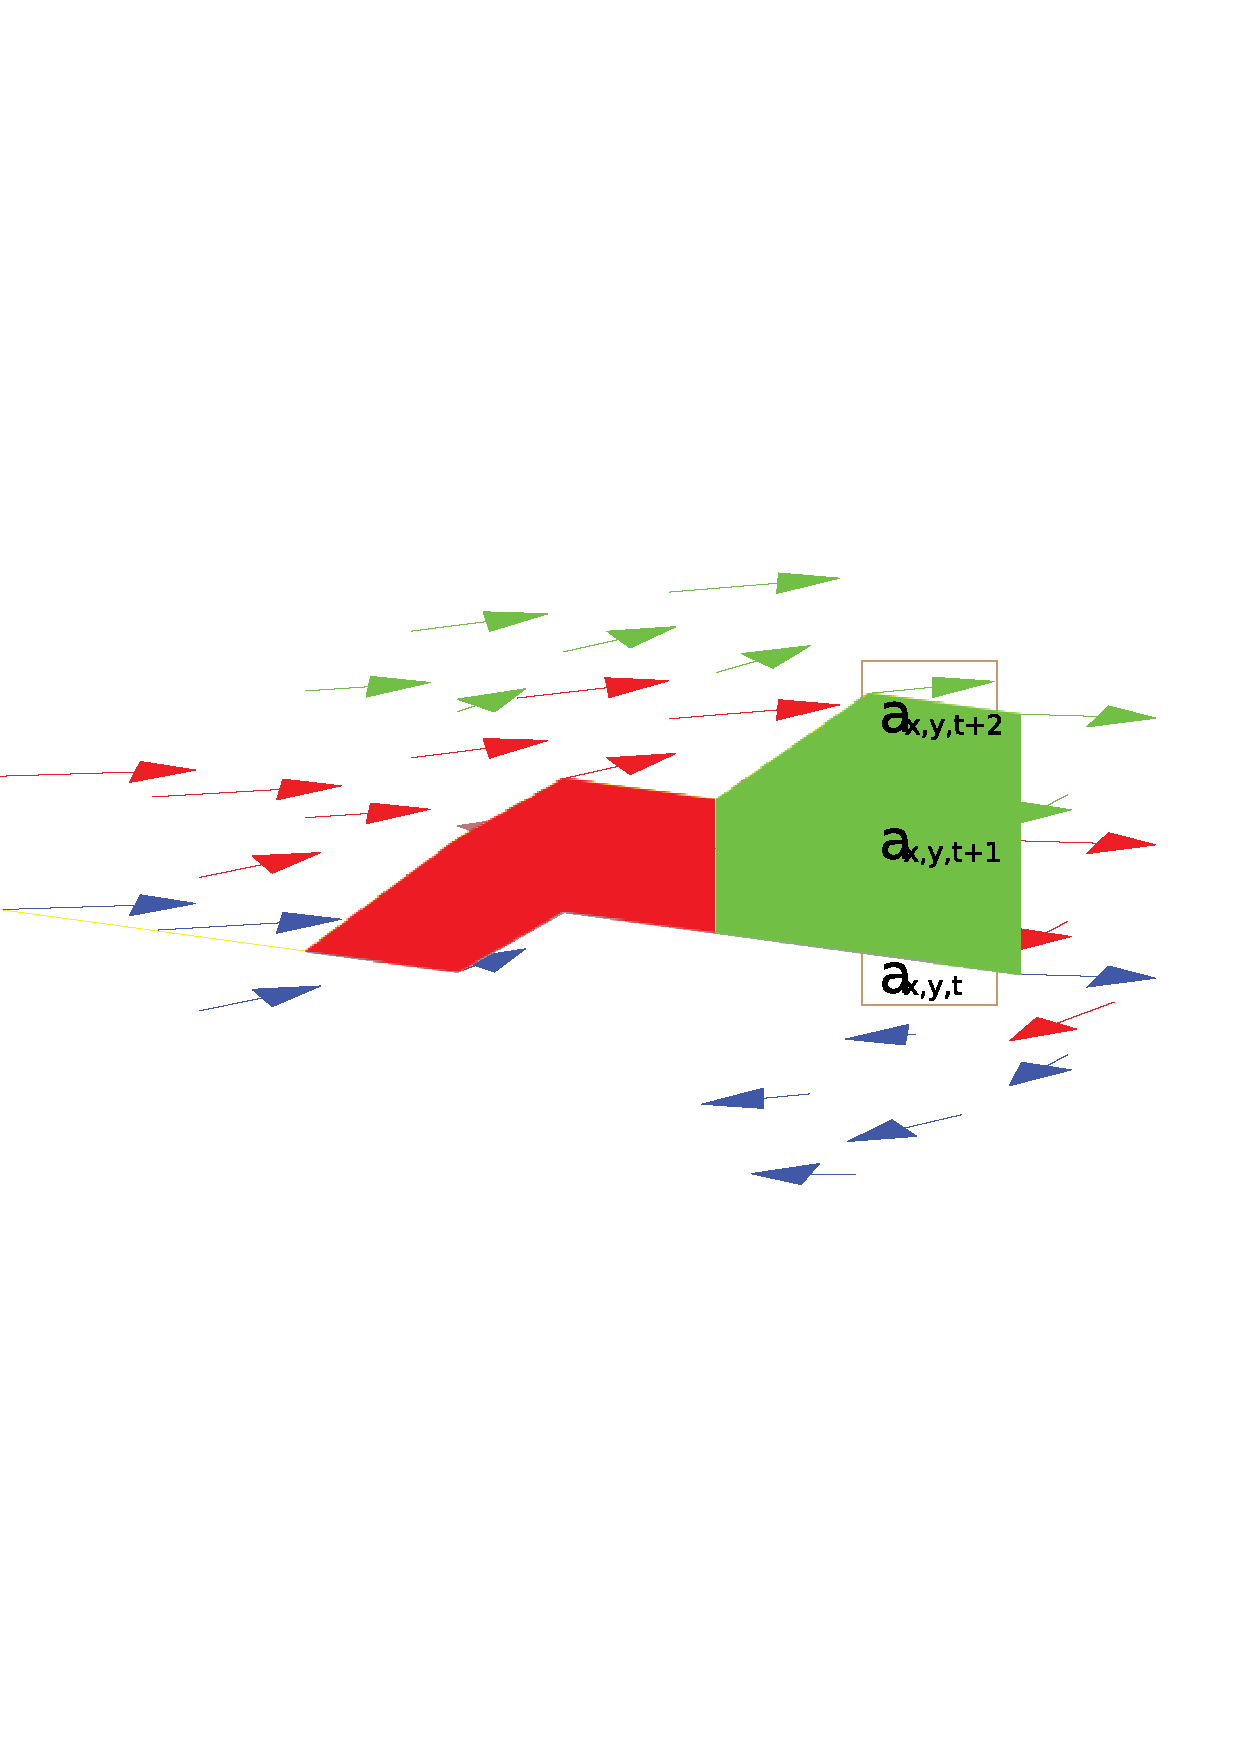
\includegraphics[width=12cm]{img/windfield-different-layer}

% Author: Mathias Hablützel

\section{Berechnung von Segelgeschwindigkeit anhand der Windfelder}
Die in Abschnitt \ref{s:windfields} eingelesenen Windfelder werden nun für die
Berechnung der Segelgeschwindigkeit verwendet. Gegen sind der
Windangriffswinkel auf das Schiff durch die Windvektoren von Punkt $A$ nach
$B$, die Segelrichtung ist damit auch bekannt.

% TODO: Skizze zeichnen mit Punkt A -> B, Segelboot, Windvektoren
 
\subsection{Geschwindigkeit am Ausgangspunkt}
Da es bekannt ist zu welcher Zeit man am Ausgangspunkt $A$ ist, weiss man auch
welcher Windvektor existiert (der sich ja mit der Zeit verändert). Somit lässt
sich die Geschwindigkeit des Bootes am Ausgangspunkt berechnen.

\subsection{Geschwindigkeit am Zielpunkt}
Hier besteht das Problem, dass es nicht bekannt ist, wann das Boot am Punkt $B$
ankommt, die Ankunftszeit hängt vom Windvektor $v_{1}$ in Punkt $A$ zur Zeit
$t_{1}$ und vom Windvektor $v_{2}$ in Punkt $B$ zur Zeit $t_{2}$ ab. $t_{2}$
ist unbekannt und folglich ist $v_{2}$ auch nicht bekannt (nur dessen Position
ist im Voraus bekannt).

Also muss in einem ersten Schritt die Ankunftszeit approximiert werden.  Wir
könnten die Euler'sche Regression verwenden, allerdings besteht hier das
Problem, dass der Algorithmus nicht zwingend die beste Lösung findet und über
eine unterschiedlich lange Laufzeit verfügt. Daher erschien ein zweischrittiges
Verfahren für eine Teilapproximation vernünftig, welches in linearer Zeit
ausgeführt werden kann.

\subsection{Berechnung der Ankunftszeit}
Vom Startpunkt $A$ ist die Uhrzeit, die Position und somit der Windvektor
bekannt. Daraus kann die Geschwindigkeit des Segelbootes bestimmt werden
(ausgehend von Punkt $A$). Diese Geschwindigkeit wird nun für die gesamte
Distanz angenommen und daraus resultiert eine ungefähre Ankunftszeit. Wir
nehmen hier an, dass das Windfeld zu einem späteren Zeitpunkt nicht so stark
ändert, dass unsere Berechnungen zu stark von einem vernünftigen Wert abweicht,
unter anderem weil dies der Natur von Windfeldern widersprechen würde.
Ausgenommen sind Extremsituationen wie Windhosen oder Tornados. Aber in solchen
Situationen wäre das Segeln auch nicht vernünftig.

\subsection{Kurs (Track)}
Die Geschwindigkeit des Segelschiffes hängt einerseits von der Intensität des Windes und andererseits von der Einfallswinkel des Windvektors ab. Damit der Einfallswinkel des Windvektors berechnet werden kann, muss bekannt sein, in welche Richtung das Segelschiff segelt. Die Berechnung des Kurses findet wie folgt statt: Zuerst wird ein Kreuzprodukt der zwei Vektoren vom Ursprung  \(\overrightarrow{A}\) und \(\overrightarrow{B}\) brerechnet. Das Resultat entspricht dann der Normalenvektor \(\overrightarrow{N}\), welche senkrecht zu der aufgespalteten Ebene von \(\overrightarrow{A}\) und \(\overrightarrow{B}\) steht. Danach wird wiederum ein Kreuzprodukt berechnet, diesmal aber vom Vektor \(\overrightarrow{A}\) und dem Normalenvektor \(\overrightarrow{N}\). Dies ergibt als Resultat die Richtung des Segelschiffes. Da dieser Vektor aber 3-dimensional ist, muss sie auf die lokale Tangentialebene (\(\overrightarrow{e_{\theta}}\), \(\overrightarrow{e_{\phi}}\)) des Punktes $A$ projiziert werden, damit wir ein 2-dimensionales Vektor kriegen. \\
Die grafische Darstellung dieser Berechnung sieht wie folgt aus:
\begin{figure}[h!]
\centering
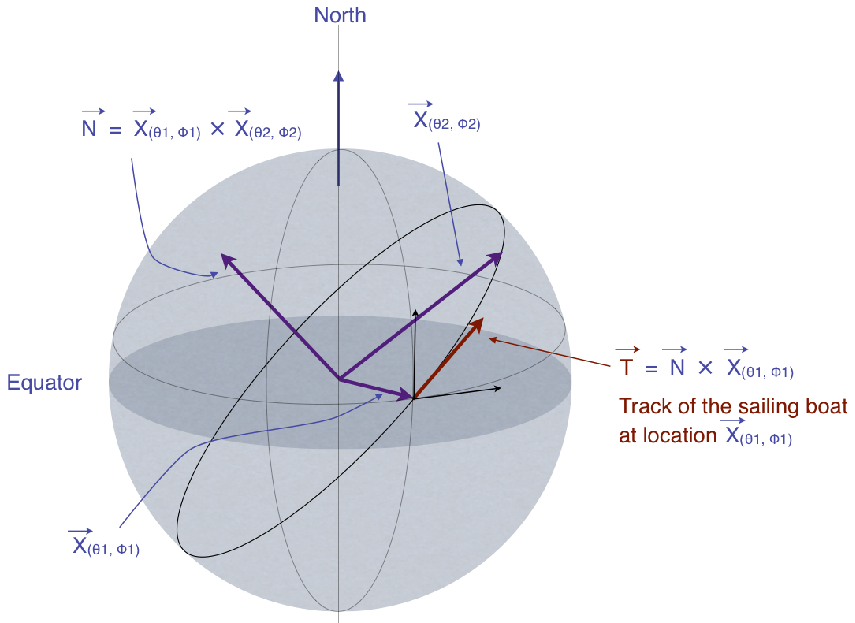
\includegraphics[width=0.8\linewidth]{img/track}
\caption{Berechnung des Kurses}
\label{gridnetConn}
\end{figure}

\subsection{Implementation}
In der Implementation haben wir einen noch einfacheren Ansatz verfolgt:

%\begin{align}
%t = \frac{1}{2} (\frac{2d}{|\mathbf{\overrightarrow{v_{1}}} + \mathbf{\overrightarrow{v_{2}}}|})
%\end{align}

% Siehe letzte SEITE vom PDF "Navigation_Commented_New.pdf"!!!!!
\begin{align}
t = \frac{2d}{\mathbf{s_{1}} + \mathbf{s_{2}}}
\end{align}

t Reisezeit, d Distanz zwischen zwei Punkten, 
$s_{1}$ bzw. $s_{2}$ Schiffsgeschwindigkeit einmal mit Windvektor $v_{1}$ und einmal mit $v_{2}$.

\vspace{0.5cm}
% Im Kapitel 9.1.1 wird es erwähnt... Hier noch ref einfügen!
Würde der Windvektor $v_{2}$ aufgrund von der absoluten Zeit, also in
Bezug zur Uhrzeit, auf das Windfeld des nächsten Zeitabschnitts fallen,
so wird $v_{2}$ mit dem des (zeitlich) nächsten Windfeldes ersetzt.







% Author: Fevzi Yükseldi

\section{Entscheidungskern}

\subsection{Problemanalyse}
\subsubsection{Erweiterung des geometrischen Entscheidungskerns}
Da der Windfeld-Container\footnote{Ein Container, der viele verschiedene Windfelder beinhaltet, auf die per Index zugegriffen werden kann.} für jede Stunde jeweils ein Windfeld beinhaltet, müssen diese natürlich auch bei der Berechnung berücksichtigt werden. Je nachdem zu welcher Zeit das Programm ausgeführt wird, soll das dazugehörige Windfeld aus dem Container herausgenommen und die Werte (die Windvektoren) davon benutzen werden. 

Wie auch schon erwähnt, wird für die Berechnung der Dauer die Windvektoren benötigt. Deswegen kann es vorkommen, dass während der Fahrt von einem Knoten zum Anderen die Windvektoren nicht mehr aktuell sind. Um dieses Problem aus dem Weg zu räumen, soll nach jeder Berechnung die Dauer überprüft werden. Falls die Dauer bis zu irgendeinem Knoten eine gewisse Grenze überschreitet, soll das Windfeld gewechselt und dementsprechend  auch die neuen Windvektoren benutzt werden. Diese Grenze befindet sich gerade in der Mitte der Zeitspanne zwischen zwei aufeinander folgenden Windfelder. 

In unserem Falle beträgt diese Grenze 30, da wir für jede Stunde ein neues Windfeld zur Verfügung haben. Somit wird bei jedem Knoten nach der Berechnung überprüft, ob die Minutenzahl der Dauer bis zu diesem Knoten kleiner oder grösser als diese Grenze ist. Falls sie kleiner ist, wird das aktuelle Windfeld beibehalten und die Berechnung fortgesetzt. Falls sie aber grösser ist, wird der Index des Windfelds um 1 erhöht und die Berechnung mit dem neuen Wert wiederholt. D.h. Der Windvektor des Zielknotens wird erneuert, wobei der Windvektor des Anfangsknotens gleich bleibt.

\subsubsection{Erstellung eines Entscheidungsbaums}
Nach den Berechnungen soll mit den Werten ein Entscheidungsbaum erstellt werden. Damit die Beziehungen zwischen den Knoten und die Dauer der Reisezeit nicht verloren gehen bzw. nicht jedesmal erneut berechnet werden sollen, wird versucht, alle nötigen Informationen in jedem Knoten abzuspeichern. Dementsprechend soll dieser Entscheidungsbaum folgende Angaben beinhalten: 
\begin{itemize}
\item Vorheriger Knoten: Die Position des vorherigen Knotens in der Form \texttt{\{i,j\}}.
\item Aktueller Knoten: Die Position des aktuellen Knotens in der Form \texttt{\{i,j\}} .
\item Dauer: Die Dauer vom Anfangsknoten bis zu diesem Knoten.
\end{itemize}
Und sieht dann grafisch dargestellt wie folgt aus:
\begin{figure}[h!]
\centering
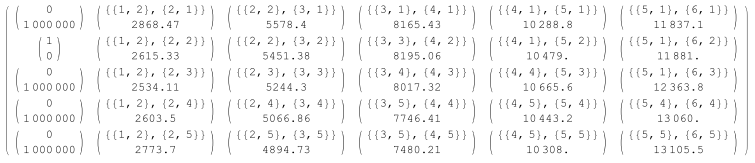
\includegraphics[width=1\linewidth]{img/grid_structure}
\caption{Struktur des Koordinatennetzes}
\label{gridnetConn}
\end{figure}


\section{GraphList}
Wie in Abschnitt \ref{aufg6:entscheidungsbaum} erklärt wurde, brauchen wir eine Liste, die alle nötigen Informationen zu den Knoten beinhaltet. Da die Grösse des Arrays variabel ist und wir zum grössten Teil einen index-basierten Zugriff benötigen, haben wir uns entschieden die Datnestruktur $java.util.ArrayList$ mit Generics zu verwenden. Eine generische ArrayList erlaubt es genau zu definieren, welche Elemente/Datentypen einer ArrayList hinzugefügt werden dürfen. Ausserdem brauchen wir für eine tabellarische Form ein 2-dimensionales ArrayList. Um dies zu erreichen, wird ein ArrayList in einem ArrayList definiert. Somit entspricht der erste ArrayList der Spalten und die zweite der Zeilen dieser Spalten. \\
Dementsprechend sieht die Initialisierung des ArrayLists so aus:

\lstinputlisting[label=src:graphListInitialization,caption=Initialisierung der Liste]{code/graphlist_initialize.java}

\subsection{Node}
Für die Speicherung der Daten wurde eine Klasse $Node$ erstellt, welche die Werte über die Knoten beinhaltet. Weil wir nun mehrere Informationen zu den einzelnen Knoten haben, haben wir uns entschieden, neben den Auflistungen in \ref{aufg6:entscheidungsbaum} auch noch weitere Daten in der Liste abzuspeichern, um Redundanz zu vermeiden. Deshalb werden neu auch Koordinaten zu den Knoten und die dazugehörigen Windvektoren in der Liste abgelegt. \\
Demzufolge enthält die Klasse folgende Informationen:
\begin{itemize}
\item \textbf{TimeOfArrival}: Die Dauer vom Anfangsknoten bis zu diesem Knoten.
\item \textbf{Previous Node}: Die Referenz zum vorherigen Knoten.
\item \textbf{Coordinate}: Breiten- und Längengrade des Knotens.
\item \textbf{WindVektor}: Der Windvektor $(u, v)$ an diesem Knoten.
\end{itemize}

Desweiteren erbt diese Klasse von der Interface $Comparable$, um Vergleiche zwischen den Knoten zu ermöglichen. Infolgedessen ist es möglich, die Klasse $Collections$ zu benutzen, welche nützliche Methoden für Listen wie $min()$, $max()$, $sort()$ etc. enthält. Wir machen in unserem Code von der $min()$-Methode Gebrauch, um den Knoten mit dem kleinsten TimeOfArrival in einer Spalte zu finden. \\

Als nächstes wurde innerhalb der ArrayList eine sogenannte LinkedList implementiert. Jeder Knoten beinhaltet eine Referenz zum vorherigen Knoten und der Anfangsknoten hat eine Referenz auf sich selbst. Dementsprechend braucht man nicht durch alle Knoten zu iterieren um einen Pfad zu zeichnen, sondern es reicht den Knoten zu wählen, von dem man den Pfad zum Anfang zeichnen möchte. \\

Die Implementation der Klasse Node sieht wie folgt aus:

\lstinputlisting[label=src:nodeClass,caption=Node-Class]{code/node.java}

\section{Polar-Diagramm}
\subsection{Parser}
Die Schiffsdaten sind als CSV\footnote{Comma Separated Values}-Datei gegeben
und werden von einem selbst\-geschriebenen Parser in ein passendes
Klassen-Konstrukt geladen. Die Schwierigkeit bestand darin, dass die Daten
nicht-dekoriert sind und daher nur durch ihre Position von anderen Typen zu
unterscheiden sind. Das bedeutet allerdings auch, dass der Parser sich auf
diese Datenstruktur verlässt und keine Abweichungen duldet und sonst abstürzt.

Dieses Problem ist allerdings vertretbar, da die Datenstruktur vorgegeben ist
und der Parser daran angepasst wurde. Es ist im Allgemeinen sehr schwierig
einen Parser für eine schwach typisierte Datenstruktur zu schreiben. Eine
robustere Datenstruktur würde XML bieten, die strikte Einschränkung bis hin zu
Datentypen für einzelne Felder bietet.

\subsection{Verarbeitungsklasse}
Die Klasse \texttt{BoatSpeedDiagram.java\footnote{Im Package
ch.zhaw.lakerouting.interpolation.boatdiagram zu finden}} verwaltet das
Polardiagram und bietet die nötigen Methoden für die Abfrage der Werte an,
kapselt die Interpolation, so das der Programmierer sich darum nicht kümmern
muss.

\subsection{Bilineare Interpolation}\label{sss:bilinearinterpolation}
Die Interpolation an sich ist durch 
\begin{equation}
f(x,y) \approx \begin{bmatrix} 1-x & x \end{bmatrix} \begin{bmatrix}
f(0,0) & f(0,1) \\ f(1,0) & f(1,1) \end{bmatrix} \begin{bmatrix} 1 - y
\\ y \end{bmatrix}
\label{eq:bilineareinterpolation}
\end{equation}
geben und kann in Java wie nachfolgend gezeigt, implementiert werden.

 \lstinputlisting[label=src:bilinearinterpolation,caption=Bilineare Interpolation]{code/BilinearInterpolation.java}
Die konkrete Berechnung erfolgt auf den Zeilen 17-19 und zeigen den einfachen
Charakter der Berechnung. Diese Implementation erfordert allerdings eine
geringe Aufbereitung der Eingabewerte, ist dafür einfacher zu testen und somit
indirekt auch weniger anfällig für Implementationsfehler, was direkt zu
robusterem Code führt.

\section{Windfelder}
Die Implementation ist vergleichsweise einfach gehalten und besteht aus einer
Klasse für ein einzelnes Windfeld mit Hilfsfunktionalitäten für die
Interpolation der Windvektoren und das Abfragen der Nachbarsvektoren an einer
bestimmten Position. Diese einzelnen Windfelder werden dann in einem Art Stapel
aufbewahrt\footnote{Wir verwenden der Einfachheit halber ein normales Array.}
Im Prinzip besteht das alles aus einer dreidimensionalen Struktur aus
Windvektoren.

\subsection{Windfeld-Parser}
Der Parser ist ein Eigenbau und wurde speziell für diese Datenstruktur
geschaffen. Diverse Unzulänglichkeiten wie nicht-leere Zeilen und Trailing
Spaces haben die Entwicklung erschwert und dementsprechend viel Zeit gekostet.

Allerdings lässt sich der Parser leicht auf andere Ressourcen erweitern wie zum
Beispiel HTTP und erlaubt auch die direkte Anbindung an Datenbanken.

\subsection{Interpolation der Windvektoren}
Da das Windfeld und das Entscheidungsnetz nicht über dieselben Koordinaten
verfügen und dementsprechend die Entscheidungspunkte normalerweise zwischen den
Windvektoren zu liegen kommen, wird nach Berechnung des Entscheidungsnetzes dem
Windfeld die Koordinatenliste übergeben. Das Windfeld interpoliert die
Windrichtung bzw. die Windvektoren an den geforderten Positionen. Das erfolgt
wie bereits in Abschnitt \ref{sss:bilinearinterpolation} erklärt über dieselbe
Klasse.

Nach dieser initialen Interpolation verfügen das Entscheidungsnetz und das
Windfeld über dieselben Array-Indizes und können somit leicht (wieder-)
verwendet werden.


\section{JavaDoc}
% Wie JavaDoc zu bedienen sei und was alles dort drin steht.

\subsection{JavaDoc}
JavaDoc ist ein von Oracle\footnote{Vormals SUN} beziehungsweise von der Java
SDK mitgelieferter Parser, der die in den Klassen geschriebene Dokumentation
extrahiert, aufbereitet und als HTML-Dokumente rendert. Es handelt sich dabei
um eine primitive Markup-Language, die HTML-Tags akzeptiert und somit dem
Entwickler die Möglichkeit geben, die Dokumentation einfach und direkt zu
beeinflussen.

So ist es möglich noch während dem Entwickeln den Sourcecode zu dokumentieren,
also wenn er noch frisch in Erinnerung ist und es wird keine wiederholte
Einarbeitung benötigt wie einer nachträglichen Dokumentation.

Wenn die Dokumentation erstellt wurde, kann mittels \texttt{javadoc} und
diversen Switches bestimmt werden bis zu welcher Detailstufe -- sollen die
private Methoden auch in die Dokumentation erscheinen -- ausgegeben werden
soll. Auch ist es möglich ein separates CSS-Files anzugeben, um die
Dokumentation der Corporate-Identity anzupassen. Nachher sind die HTML-Dateien
bereit für die Publikation auf dem Webserver des Projektes.

\begin{center}
\begin{minipage}[c]{0.5\linewidth}
 \centering
 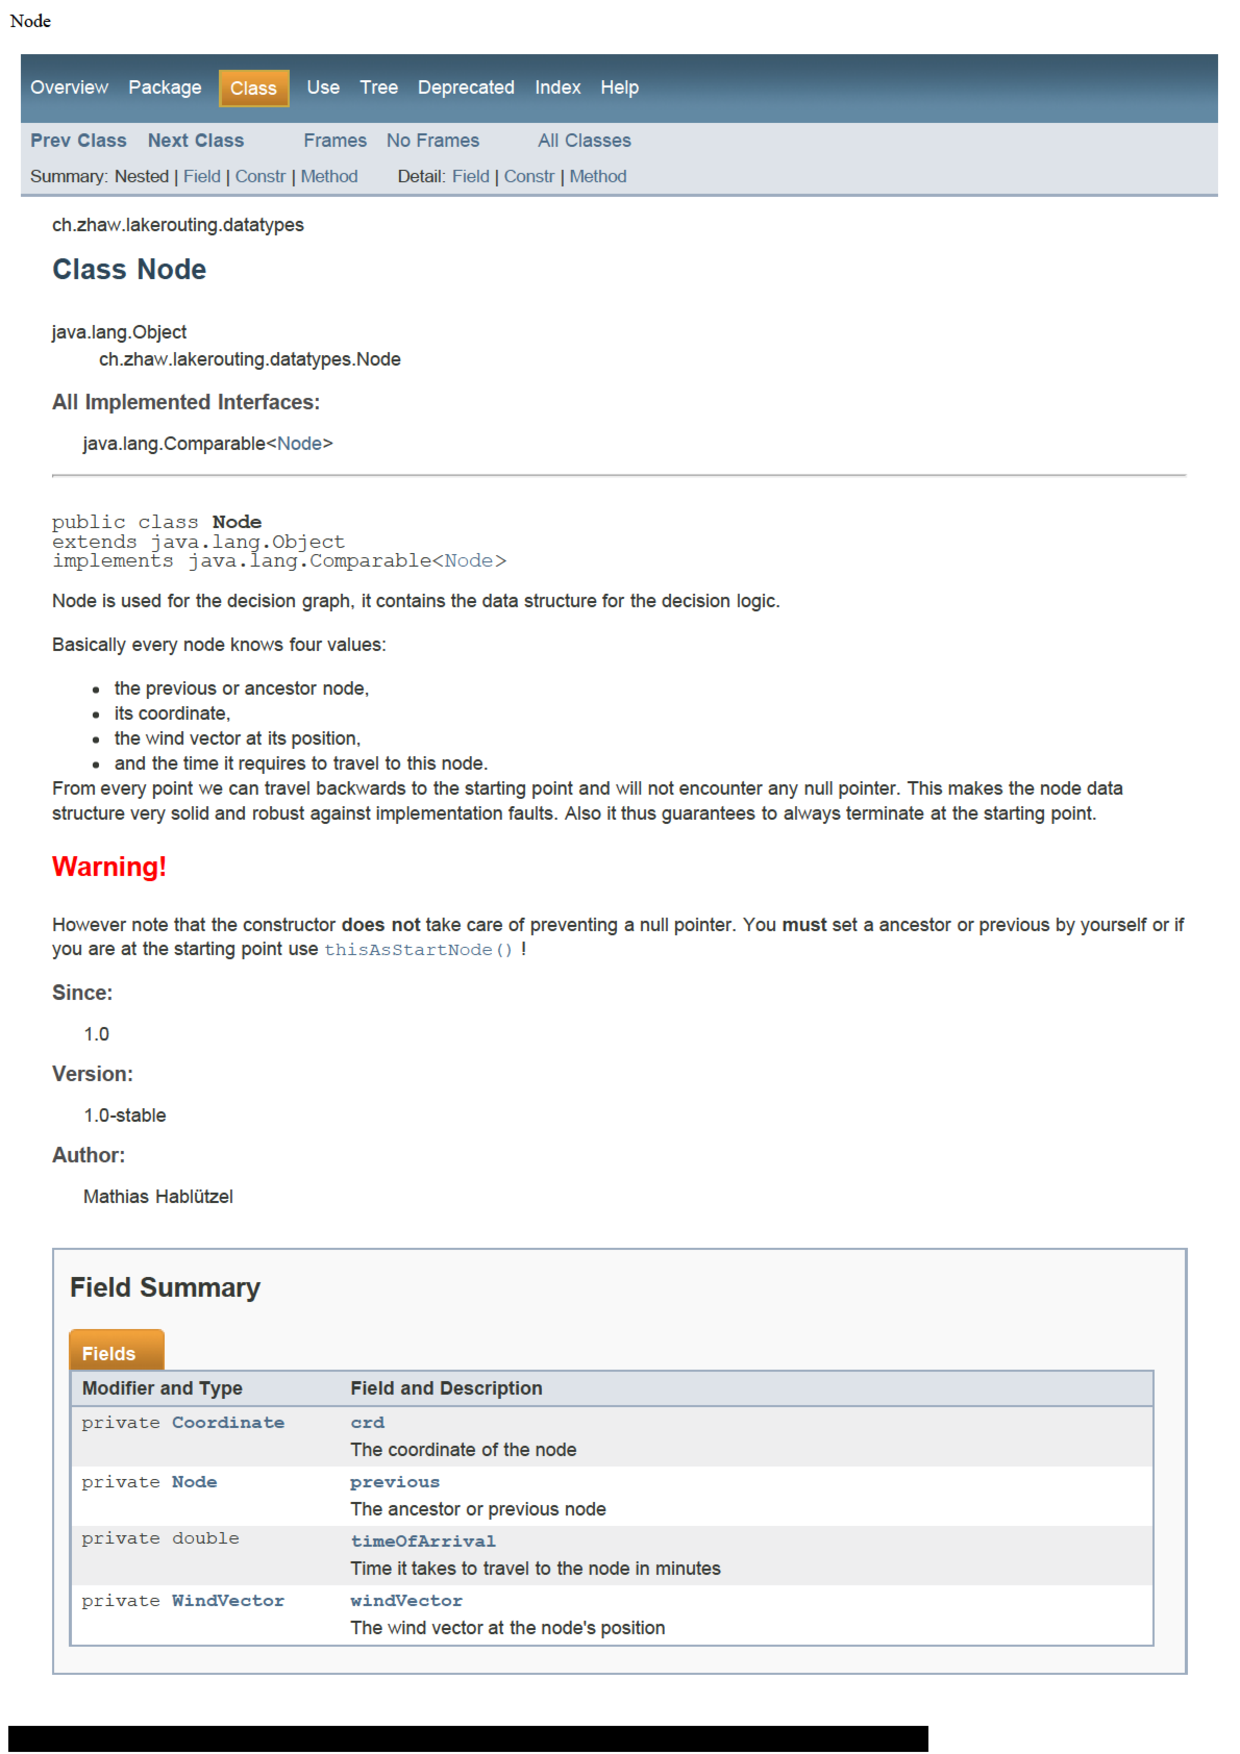
\includegraphics[width=\linewidth]{img/javadoc-screenshot.pdf}
\end{minipage}
\end{center}


\section{Testing}
Um die Applikation auf Erfüllung der für ihren Einsatz definierten
Anforderungen zu bewerten und zu prüfen sind Softwaretests nötig. Es wurde
versucht, diese Tests am Anfang zu erstellen und im Laufe der Entwicklung
regelmässig zu durchführen und erweitern. Es wurden in der Regel zwei Arten
von Tests eingesetzt: manuelle und automatisierte Tests. Die manuellen Tests
wurden einerseits mit dem Debugger zur Verifizierung der Inhalte und
andererseits mit systematisch festgelegten Eingabedaten ausgeführt. Daneben
wurden auch noch die automatisierten Unit-Tests eingesetzt, um zu
verifizieren, dass bei Änderungen keine unerwünschten Nebeneffekte
hervortreten. 

In unserer Appkilation wurden für alle Packages mindestens ein JUnit-Test
geschrieben. Es wurden entweder ganze Klassen oder nur gewisse, essenzielle
Methoden getestet. Somit sollten diese Tests die meisten Fällen abdecken. 

\subsection{JUnit Test}
JUnit ist ein kleines, mächtiges Java-Framework zum Schreiben und Ausführen
von automatisierten Unit-Tests. Es werden in der Regel für alle Klassen, die
überprüft werden sollen, ein Unit-Test erstellt. Diese Unit-Tests verhalten
sich auch wie die gewöhnlichen Java-Klassen, mit dem Unterschied, dass sie im
Namen das Wort \texttt{Test} am Schluss und einige JUnit-Annotationen innerhalb der
Klasse haben, wobei die Endung im Namen nur eine Konvention ist. Ein
JUnit-Test kennt nur zwei Ergebnisse: Entweder war der Test erfolgreich oder
nicht. Das Fehlschlagen kann zwei Gründe haben, entweder war es ein
Fehler(Error) oder es lieferte ein falsches Ergebnis (Failure). Der einzige
Unterschied zwischen den beiden Begriffen liegt darin, dass Errors eher
unerwartet auftreten, während Failures erwartet werden. Desweiteren können die
geschriebenen Testfälle zu jeder Zeit beliebig wiederholt werden. 

Ausserdem bietet dieses Framework einige Methoden an, um Werte vergleichen zu
können. So zum Beispiel vergleicht die Methode \texttt{assertEquals(expected, actual,
delta)} zwei Werte, expected und actual, und kann eine Abweichung beinhalten. 

\subsubsection{Beispiele}
% Mit sinnvollen Beispielen simulieren.
Als Beispiel für ein JUnit-Test kann der Test für die Klasse $TrackComputation$ gebracht werden. 
Diese Klasse berechnet den Winkel zwischen zwei Punkten $A$ und $B$. Für die Berechnung
wurden simple Beispieldaten genommen, um das Resultat auch selbst nachvollziehen zu können.
Diese Daten wurden in einer $HashMap$ gespeichert. Ein $HashMap$ ist ein Assoziativspeicher. 
D.h. dass diese Klasse Datenelemente mit Schlüssel und Wert-Paaren abspeichert. In unserem
Beispiel fungiert sie eher als eine Liste. Danach werden diese Werte ausgelesen und der 
Winkel berechnet. Falls die berechneten Winkel mit den $Mathematica$ Lösungen übereinstimmen,
war der Test erfolgreich (grün).

Der JUnit-Test sieht wie folgt aus:

\lstinputlisting[label=src:trackComp,caption=JUnit-Test für die Klasse TrackComputation]{code/trackComputationTest.java}

Da der Windfeld-Container mehrere Windfelder hat, wurden auch einige Simulationen 
zur besseren Veranschaulichung und der Nachvollziehbarkeit durchgeführt. Es wurde versucht,
möglichst verschiedene Routen berechnen und zeichnen zu lassen, um die Korrektheit des
Algorithmus aufzuzeigen. 

Das erste Beispiel soll aufzeigen, wie die optimale Route einen Zick-Zack Kurs einnehmen muss,
um am schnellsten am Ziel anzukommen:

\begin{figure}[h!]
\centering
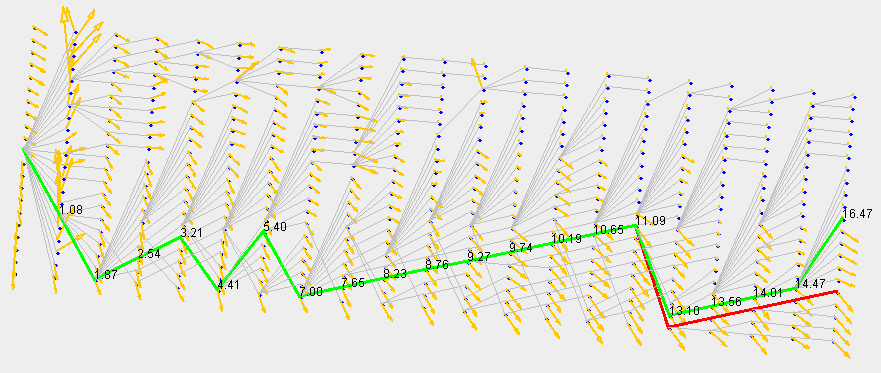
\includegraphics[width=0.8\linewidth]{img/gridNet_1}
\caption{Zick-Zack Kurs für die optimale Lösung.}
\label{gridnet1}
\end{figure}

Dieses Beispiel zeigt eine primitive und glatte Lösung, da die Windvektoren schon einigermassen in diese Richtung zeigen:

\begin{figure}[h!]
\centering
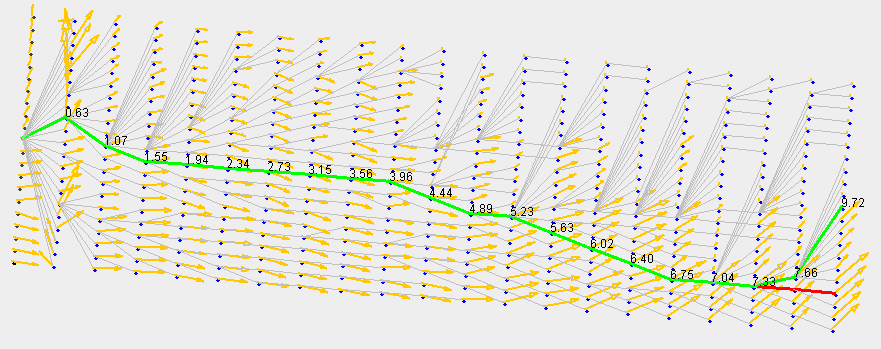
\includegraphics[width=0.8\linewidth]{img/gridNet_2}
\caption{Primitiver und glatter Kurs für die optimale Lösung.}
\label{gridnet1}
\end{figure}

Als letztes Veraunschaulicht dieses Beispiel eine Route, die ihren Kurs in der Mitte ziemlich ändern muss, da die Richtungen der Windvektoren sich umgekehrt haben. 

\begin{figure}[h!]
\centering
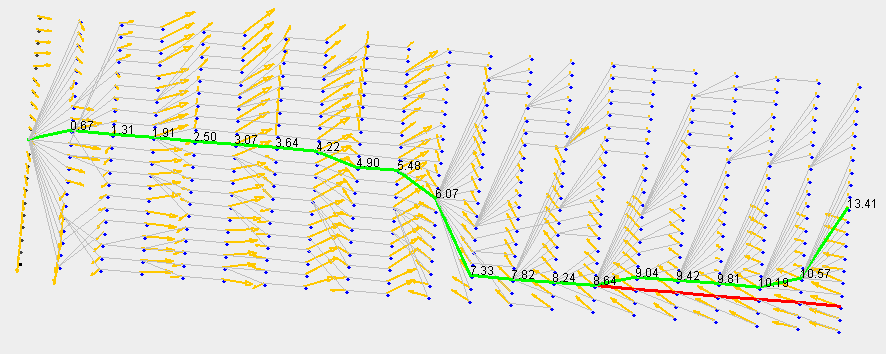
\includegraphics[width=0.8\linewidth]{img/gridNet_20}
\caption{Änderung des Kurses in der Mitte für die optimale Lösung.}
\label{gridnet1}
\end{figure}


\newpage
\part{Diskussion und Ausblick}
% Interpretation und Validierung der Resultate
% Author: Mathias Hablützel
% Interpretation und Validierung der Resultate

\section{Erweiterbarkeit}
% Zeigen, dass es leicht erweiterbar und wiederverwendbar ist.
\subsection{Wiederverwendbarkeit}
Java ist eine strikt objektorientierte Sprache und zwingt den Entwickler
Klassen zu entwickeln. Allerdings bedeutet das nicht, dass dadurch automatisch
auch modularer und wiederverwendbarer Code entsteht. Durch das geschickte
verwenden von Entwicklungsmustern kann man schon früh in der Planungsphase
sicherstellen, dass möglichst wiederverwendbarer Code entsteht. Ein gutes
Anschauungsbeispiel ist hier die Klasse \texttt{Bilinear.java}, dass eine
Implementation des Interfaces \texttt{InterpolationAlgorithm.java} ist. Das
Interface gibt einzig vor, welche Schnittstellen beziehungsweise welche
Methoden zu implementieren sind und in unserem Fall auch andere gewisse
Randbedingungen. Somit kann die Klasse für Interpolation einfach ausgetauscht
werden mit einem anderen Algorithmus, ohne das der Rest der Software betroffen
ist. Somit wäre es möglich komplexere Interpolationsverfahren zu nutzen, die
zum Beispiel spezialisierte Hardware wie ein FPGA\footnote{Field-programmable
gate array}, um eine noch schnellere Berechnung grosse Datensätze zu
ermöglichen.

\subsection{Parallelisierung}
% Aufzeigen, dass Paralellisierung möglich ist.
\subsubsection{Multi-Core-CPU}
Im Rahmen der Arbeit hat sich schnell die Frage gestellt, wie man die
Multi-Core-Architektur eines Supercomputer ausreizen kann. Die jetztige
Implementation verwendet eine reine Single-Thread-Archtitektur mit synchronen
Aufrufen. Das bedeutet einerseits, dass die nominelle Taktgrösse der CPU die
Verarbeitungsgeschwindigkeit direkt bestimmt und andererseits liegen die
anderen Cores brach und werden nicht benutzt. Da aber heute immer mehr CPUs
mit tieferen Taktraten dafür mehr Cores gebaut werden, vergeuden wir
eigentlich viel Leistungspotential.

Allerdings muss auch beachtet werden, dass solange die TDP\footnote{Thermal
Design Power, maximale Verlustleistung} nicht verbraucht wird, sich die
ungenutzten Cores abschalten und damit dem aktiven Core erlauben zu übertakten
und die verfügbare Verlustleistung auszureizen.  Jedoch muss erwähnt werden,
dass die Verlustleistung nicht linear mit der Rechenleistung zunimmt und es
damit kein sinnvoller Trade-Off darstellt, insbesondere wenn dadurch höchsten
30\% mehr Berechnung drin liegen gegenüber 400\% bei voller
Quad-Core-Berechnungen.

\subsubsection{Asynchronous Threads}
Auf der anderen Seite blockieren wir mit synchronen Methodenaufrufe die
Reaktionsfähigkeit der Benutzerinterfaces. Das heisst, dass der Benutzer ein
eingefrorenes Programm sieht, solange die Algorithmen beschäftig sind. Solche
Oberflächen gehören zu den Tabu-Design-Prinzipien: Ein Programm sollte dem
Anwender immer über seinen internen Zustand informieren und wissen lassen wie
weit seine Berechnungen schon getätigt wurden. Ein Benutzer könnte eine nicht
reaktive Oberfläche so missinterpretieren, dass die Software abgestürtzt ist,
sein Beenden erzwingt und die Berechnung unsinnigerweise von neuem anstösst.

Somit wäre es sinnvoll Threads mit Callback-Hooks zu erstellen, die in
regelmässigen Berechnungsabständen ihren Status melden. Wichtig ist hier, dass
die Häufigkeit von Rückmeldungen nicht von Timern also zeitabhängig ist. Viel
sinnvoller ist es, nach einer Anzahl von Operationen den Stand der
Berechnungen zu melden. Eine übliche Vorgehensweise ist die Anzahl
Berechnungen zu ermitteln und bei jedem Abschluss der Berechnung diese als
erfolgt zu markieren.

\subsubsection{MapReduce}
MapReduce\footnote{MapReduce ist eine Entwicklung von Google und ist als
Hadoop Mapreduce in einer OpenSource-Fassung verfügbar.} ist eine sehr
effiziente Möglichkeit für Clustercomputing die maximale
Berechnungsgeschwindigkeit zu verwenden. Das Problem wird solange in seine
Teilprobleme zerlegt, bis entweder jeder Knoten im Cluster beschäftigt ist
oder das Problem nicht mehr zerlegt werden kann. Danach werden die Resultate
wieder eingesammelt und der aufrufenden Komponente
bereitgestellt.\cite{Google:MapReduce}

\subsubsection{GPGPU\protect\footnote{\textbf{G}eneral-\textbf{p}urpose computing on \textbf{g}raphics \textbf{p}rocessing \textbf{u}nits}}
Eine weitere Stufe des Parallelisierung wäre das Verwenden von einer
Grafikkarte, die mit ihren vielen Shader-Kerne sehr viele Berechnungen
parallel ausführen kann. Insbesondere verfügen die Grafikkarten über solche
speziellen Interpolations-Stufen und können auch komplexere
Interpolationsalgorithmen in sehr kurzer Zeit ausführen.
 
\subsection{Weitere Datenquellen}
% Wie weitere Datenquellen eingesetzt werden können (z.B. HTTP anstatt Datei)
Zu einer späteren Zeit wäre es möglich die Informationen über Windfelder und
des Polardiagramms per HTTP oder andere Protokolle zu laden. Somit wäre es
möglich die aktuellen Windfelder von einem zentralen Server zu laden, der an
einem anderen physischen Standort ist, ohne per NFS darauf zuzugreifen.

\subsection{Website}
% Wie daraus eine Webseite gemacht werden kann. Apps?
Sobald die Applikation in die Infrastruktur der MeteoSchweiz integriert ist,
wäre die kommerzielle Verwendung mit einer Website oder über eine Mobile-App
eine interessante Bachelor-Arbeit. Der Benutzer würde dann zum Beispiel per
Mobile-App seine aktuelle Position mitteilen, sein Bootstyp auswählen und
seine Zielkoordinaten. Diese werden dann an den MeteoSchweiz-Server
übermittelt und die Berechnung angestossen. Die Resultate können dann entweder
als grafische Karte oder als Datei mit GPS-Koordinate ausgegeben werden. Da
die meisten Smartphones Google Maps installiert haben, können diese sehr
einfach das GPX-Dateiformat verwenden und die Route als Overlay darstellen.

\subsection{Isochronen}
Die Isochronen bezeichnen die Verbindungslinien der verschiedenen Routen, die
von einem Anfangspunkt aus in derselben Zeit zu erreichen sind.  Für die
Umsetzung dieser Erweiterung sollte eigentlich eine Dreisatz-Berechnung
genügen. Da wir zu jedem Knoten die Dauer der Fahrt haben, braucht man nur
noch festzustellen, zwischen welchen Spalten diese Zeit der Isochronen zu
kommen hat. Nachdem dies berechnet wurde, wird anhand der Länge der Strecke
zwischen diesen beiden Spalten ein Dreisatz gebildet, welches uns die Länge
bis zum Isochron liefert. Zum Schluss brauchts nur noch den Punkt zu zeichnen.

Umgesetzt sollte es ungefähr so aussehen:

\begin{figure}[h!]
\centering
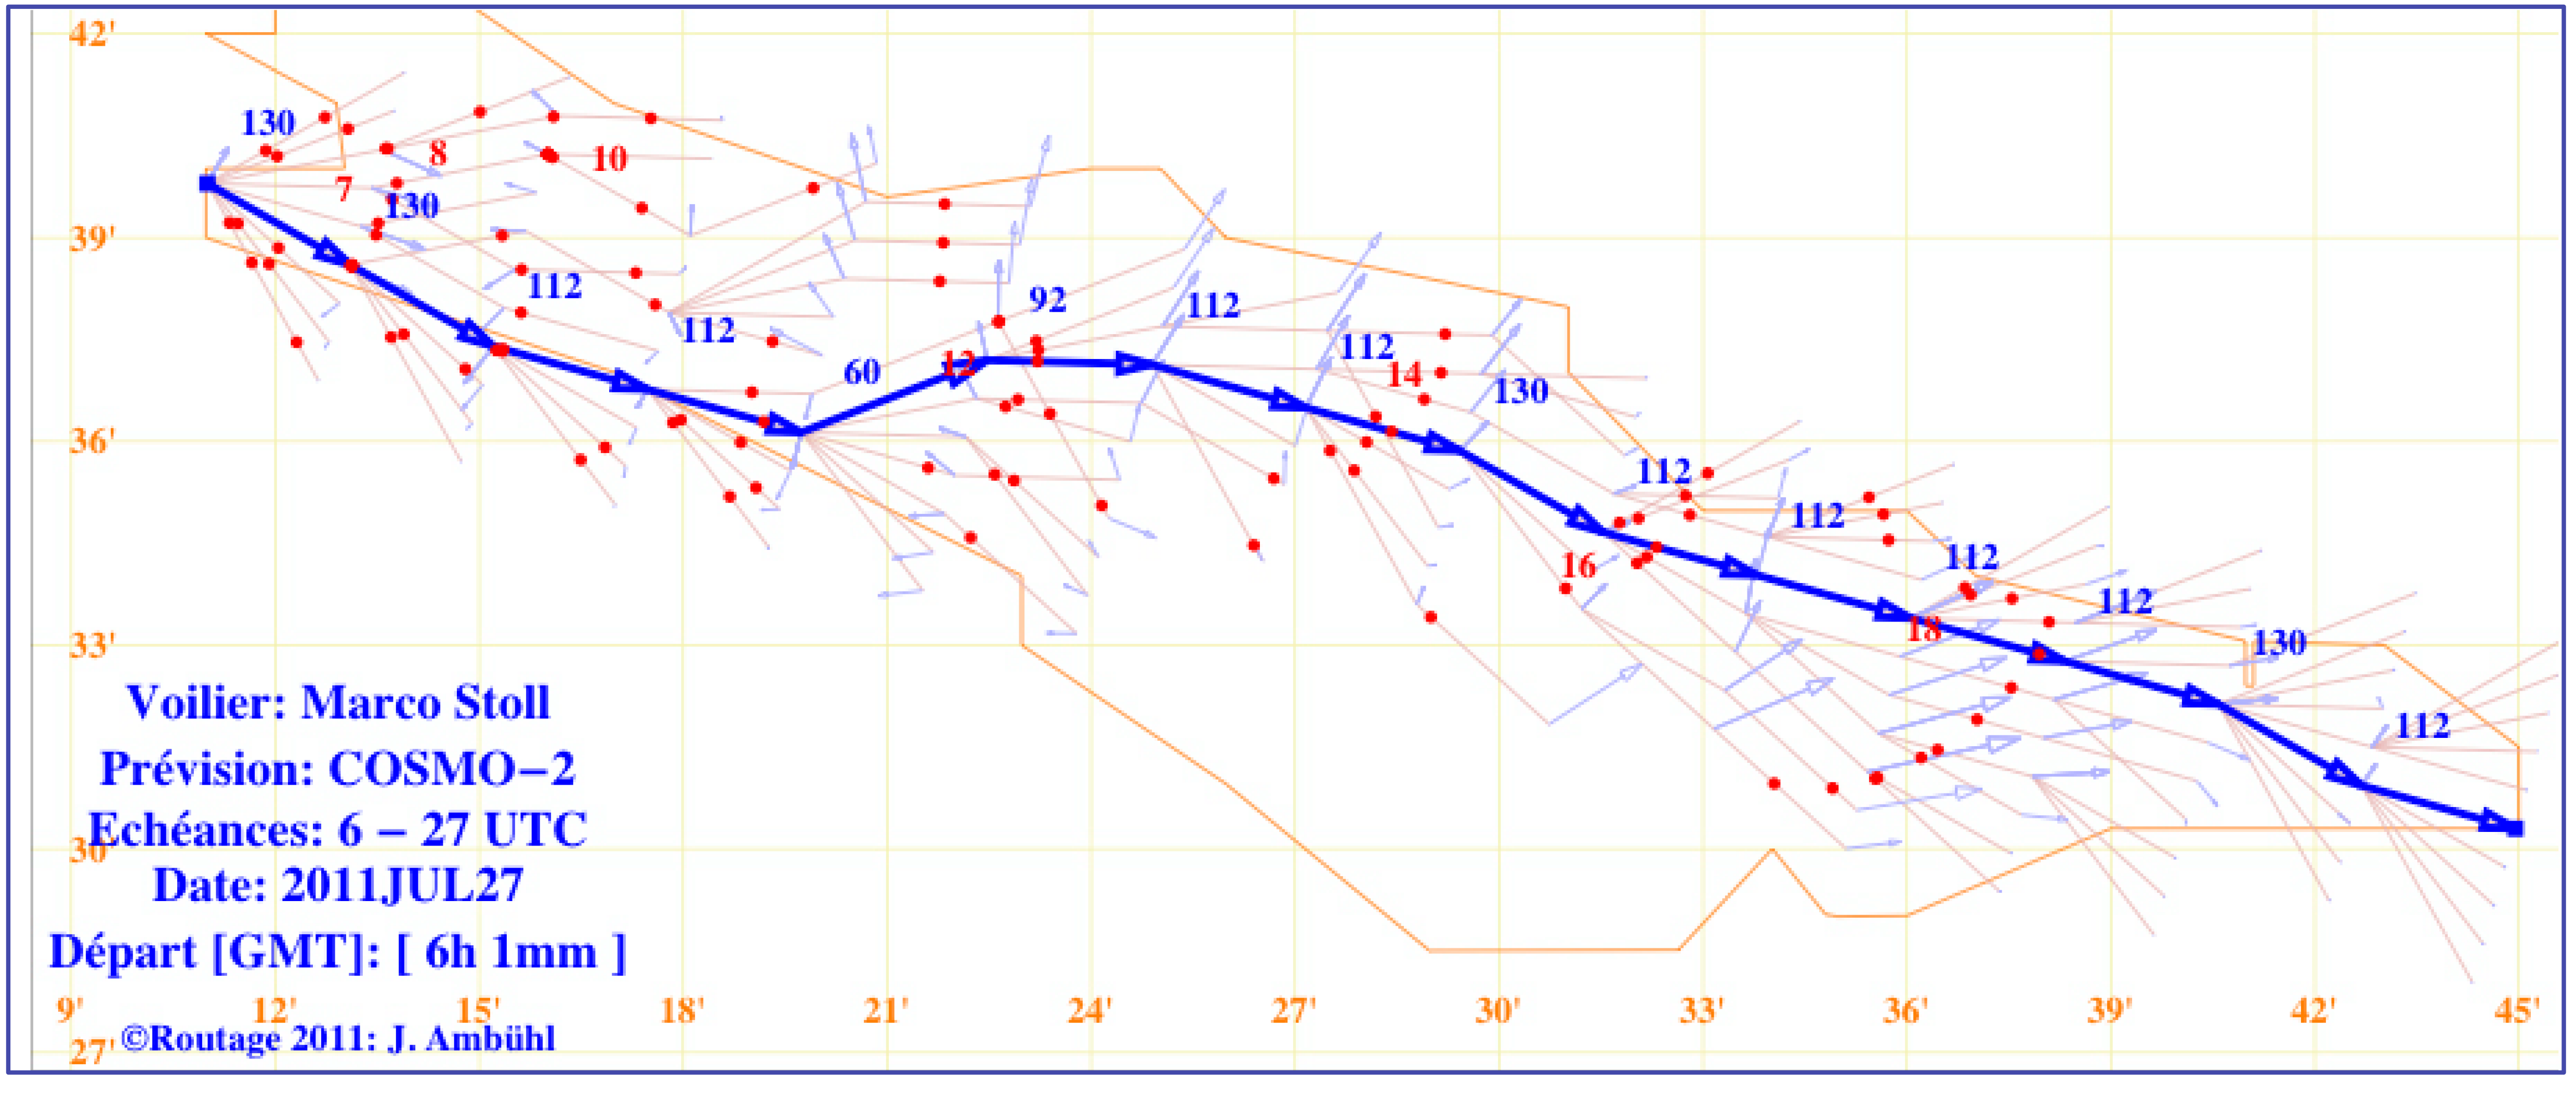
\includegraphics[width=1\linewidth]{img/isochronen}
\caption{Isochronen zu gegeben Zeiten}
\label{isochron}
\end{figure}

\section{Programmiertechnische Grenzen}
% (Im Sitzungsprotokoll vom 06.03.2012, Punkt 3)
%% 3. Im Bericht sollte ein Absatz vorhanden sein, welches die 
%% programmiertechnischen Grenzen oder Genauigkeiten der mathematischen 
%% Funktionen wie Sinus/Cosinus, Datentypen etc. behandelt und diskutiert. 
\subsection{Double-Genauigkeit}
Intern verwendet Double die \texttt{IEEE 754}-Arithmetik und beschränkt damit
die Genauigkeit der Zahlen und Berechnungen. Allerdings reicht die Genauigkeit
für unsere Zwecke zu genüge aus, da wir nie in einen Grenzbereich des
Double-Datentyps kommen. Die kleinste Zahl für die Windgeschwindigkeit ist ja
auf $0.0001$ limitiert worden. Unvernünftig grosse Werte erwarten wir sowieso
nicht, somit stellen diese Beschränkungen keine Probleme dar.

\subsection{Berechnungsgenauigkeit von primitiven Mathematikfunktionen}
Intern werden die die Resultate für die Sinus- und Cosinus-Funktionen in
Lookup-Tabellen abgespeichert und bei der Abfrage durchlaufen. Da wir nicht
eine Präzision von mehreren Nachkommastellen benötigen, reicht die vorhandene
Präzision. Dazu kommt, dass ein Segelboot unter keinen Umständen den Kurs auf
zwei Nachkommastellen halten kann.

\section{Sonderfälle}
\subsection{Unvollständiger Entscheidungsbaum bei zu kleinem Spread-Faktor}
Es ist ein Fall bekannt, bei denen die Berechnungen zwar korrekt terminieren,
aber der Entscheidungsbaum unvollständig wird. Für den Knoten \texttt{k} wird
nun der optimale Vorgänger berechnet und gespeichert sofern dieser innerhalb
des angegebenen Spread liegt.

Allerdings könnte ein Spezialfall eintreten, bei dem der letzte
Vorgängerknoten der optimale Vorgänger ist, allerdings ausserhalb des Spreads
liegt. Dann wird dieser nämlich als optimaler Vorgänger gespeichert mit
\texttt{MAX\_TOA} als Adjazenzgewicht. Allerdings scheitert wird die Abfrage
in Zeile \ref{sloc:verifyspread} des Listings \ref{lst:decisionspreadbug} und
der Vorgänger wird nicht in \texttt{GraphList} gespeichert, was zu einem
Knoten ohne Vorgänger führt und damit zu einem NullPointer.

\begin{lstlisting}[caption={Schwer zu findender Bug in
Decision.java},label=lst:decisionspreadbug,escapeinside={@}{@}]
for (int j = 0; j < getMaxj(); j++) {
        travelDistance[j] = calcTravelDistance(r, j, k, windfieldNo);
        
        /*
         * Saves the minimum distance and makes sure that the node is in
         * the spread.
         */
        if (travelDistance[j] < maxTimeOfArrival) {
        	/*
        	 * Checks, if the position of the shortest distance is legal
        	 * based on spread. If not, it sets the default distance.
        	 */
        	if (Math.abs(k - j) <= spread) {
        		maxTimeOfArrival = travelDistance[j];
        		position[k][__ROW__] = j;
        		position[k][__TRAVELTIME__] = travelDistance[j];
        	} else {
        		position[k][__ROW__] = j;
        		position[k][__TRAVELTIME__] = MAX_TOA;
        	}
        }
}

@\label{sloc:verifyspread}@ if (Math.abs(k - (int) position[k][__ROW__]) <= spread) {
       /*
        * SNIP
        */
       graphList.get(r).get(k).setTimeOfArrival(position[k][__TRAVELTIME__]);
       graphList.get(r).get(k).setPrevious(graphList.get(r - 1).get((int) position[k][__ROW__]));
}

\end{lstlisting}

\subsection{Falsche Hysterese-Berechnung}
Ein weiterer schwer zu findender Bug ist eine unvollständige
Hysterese-Berechnung in \texttt{Decision.java}. Wie Listing
\ref{lst:hysterisisbug} zeigt, wird berechnet um wie viele Windfelder der
Algorithmus in der Zeit nach vorne springen soll, wenn die Reisezeit mehr als
30 Minuten beträgt. Nehmen wir also an, die Reisezeit
(\texttt{\_\_TRAVELTIME\_\_}) würde nun 40 Minuten betragen, dann erhalten wir
richtigerweise einen Sprungwert von 1. Nehmen wir nun eine Reisezeit von 70
Minuten an, würde der Sprungwert 2 betragen, obwohl für eine Reisezeit von
30--90 Minuten der Sprungwert 1 betragen soll.
\begin{lstlisting}[caption={Hystereseberechnung in Decision.java},label=lst:hysterisisbug]
private static final double TIME_LIMIT_OF_WF = 30d;
     /* SNIP */
int windField_raise = (int) (position[k][__TRAVELTIME__] / TIME_LIMIT_OF_WF);
\end{lstlisting}

\subsection{Wrap-around-Problem beim Äquatorüberschreiten}
Die Orthodromie ist immer die kürzeste Route zwischen zwei Punkten auf einer
Sphäre. Nehmen wir als Beispiel eine Regatta von Spanien via Australien nach
Hawaii an. Die Orthodromie würde nun besagen, dass es westwärts -- also via
Amerika -- schneller wäre, obwohl das Entscheidungsnetz ostwärts zeigt. Somit
laufen wir in ein Wraparoundproblem bei den Zahlen rein. Die Software
funktioniert für die geforderten Zwecke (keine Vorzeichenwechsel bei den
Koordinaten) aber wie gewünscht. Eine Verwendung für transatlantische
Segeltörns oder Äquatorquerungen bedarf einer gründlichen Überprüfung von
Extrem- und Grenzwertkriterien.

\section{Erkenntnisse}
\subsection{Schlussfolgerung}
Mit der dynamischen Programmierung ist es möglich komplexe Probleme effizient
und elegant zu lösen, selbst wenn die Randbedingungen Ringabhängigkeiten
bilden. Sobald der Kernalgorithmus stabil implementiert ist, kann man einfach
die Daten für die grafische Darstellung extrahieren. Der Vorteil von der
dynamischen Programmierung ist die Möglichkeit das Problem so aufzuteilen,
dass es verteilt läuft und bei einer grossen Anzahl von Berechnungen auch auf
einem Cluster skaliert.

\subsection{Arbeitsrevue}
Wie bei jeder Gruppenarbeit ist es typisch, dass unterschiedliche
Erfahrungsniveaus, Programmierfertigkeiten und Vorwissensstände
aufeinandertreffen. Doch bei dieser Arbeit war es erstaunlich wie selbst die
Vorlieben für gewisse Programmiersprachen keinen Einfluss auf die Fertigkeiten
des Schreiben von Parser und Algorithmen hatten.

Problematischer war allerdings die Tatsache, dass Windows nicht durchgehend
ein UTF-8 als Charset verwendet und sich das im Repository durch falsche
Dateinamen manifestierte. Auch war \texttt{git} eine Herausforderung, die
allerdings sich dann als ein mächtiges und äussert flexibles
Source-Code-Verwaltungs-System herausstellte.

Als förderlich stellte sich eine flache Hierarchie und kurze
Kommunikationswege heraus. Da neben den Zielen kaum Einschränkungen oder
Vorgaben gemacht wurden, konnten Design-Entscheidungen völlig frei getätigt
werden, was auch Aufgrund der Erfahrung zu besseren Lösungen führte als in der
Beispielimplementation.

\newpage
\part{Anhang}

\section{Projektplanung}

\subsection{Projektübersicht}

\subsubsection{Benötigte Ressourcen}
\begin{itemize}
\item Menschliche Ressourcen \\
Das Projekt wird von 2 Personen für rund 1 Semester mit der Betreuung
eines Dozenten gemäss dem Auftrag des Auftraggebers durchgeführt. Auch
seitens des Auftraggebers steht ein Betreuer zu Verfügung, den wir bei
Unklarheiten ebenfalls kontaktieren können und von dem wir auch die
nötigen Unterlagen zugeschickt bekommen. Ausserdem steht auch ein
Nebenbetreuer zur Verfügung, der grundsätzlich für IT spezifische Fragen
zuständig ist. Es wird davon ausgegangen, dass alle Projektmitglieder
durchschnittlich 20 bis 25 Stunden pro Woche am Projekt arbeiten.

\item Räume \\
Es werden keine speziellen Räume gebraucht. Aber für eine bessere,
verstärkte und erfolgreiche Zusammenarbeit wurde das Zimmer TE616 in der
ZHAW-Schulgebäude reserviert. Ausserdem werden einmal die Woche, jeweils
am Dienstag, zwei Zimmer der Abteilung Wetterdienst in der
MeteoSchweiz-Gebäude benutzt. Jedoch wird das Projekt weitgehend als
virtuelle Organisation geführt, das heisst, dass der physische Standort
der Teilnehmer nicht von Bedeutung ist.

\end{itemize}

\subsubsection{Meetings}
Die Kommunikation im Projekt mit den beiden Betreuer erfolgt in Form von ordentlichen Meetings jeden Dienstag in der Hauptgebäude der MeteoSchweiz in Zürich. Bei Bedarf kann sie auch per E-Mail oder ausserordentlichen Sitzungen stattfinden. Ausserdem wurde für das Projekt 4 Meilensteine definiert, welche dann anstelle der wöchentlichen Sitzungen stattfinden werden. Die Meilensteine liegen bewusst vor dem eigentlichen Abgabetermin, um Pufferzeiten zu schaffen.

\subsubsection{Kontaktdaten des Auftraggebers}
MeteoSchweiz\\
Eidgenössisches Departement des Innern EDI \\
Bundesamt für Meteorologie und Klimatologie\\
Krähbühlstrasse 58\\
CH-8044 Zürich\\
Tel.   +41 44 256 91 11 \\
Fax   +41 44 256 92 78\\

\subsection{Vorgehensmodell}
%Unvollständig
Für unser Projekt haben wir uns für das V-Modell entschieden, da die
Phasen stabile Anforderungen haben und sie wenig Management-Aufwand
benötigen. Desweiteren besitzen sie klare Abgrenzungen und der Umfang
der Arbeit ist klar abschätzbar. Ein weiterer Vorteil des V-Modells für unser 
in Arbeitspakete unterteilten Projekt ist das Testing, somit ist es möglich, die 
Applikation jederzeit zu testen und dadurch jederzeit zwischen 
der Implementierung und dem Testing zu wechseln.

\subsection{Zeitliche Planung}
%120 Tage insgesamt soll es sein 78+10=88 +2 = 90 + 15= 105    10+15+78-5=108+12=120
%12+8+25+10=55+13=68    90+5+17+20=42
\subsubsection{Effektiver Ablauf}
\begin{table}[h!]
\centering 
  \begin{tabular}{| c | l | r | >{\color{red}} r |}
    \hline
    \rowcolor{hellgrau} 
    \textbf{Arbeitspakete} & \textbf{Tasks} & \textbf{Zeitaufwand} & \textbf{\color{black}Effektiv} \\ \hline \hline
    \multirow{1}{*}{} & \textbf{Planung} & \textbf{ 5 Tage} & \textbf{ 5 Tage}  \\ \cline{2-4} \hline \hline
     & \textbf{Implementierung} & \textbf{ 72 Tage} & \textbf{ 89 Tage}  \\ \hline
     \multirow{1}{*}{Nr. 1}& Aufgabe 1+2 & 12 Tage & 12 Tage \\ \hline
     Nr. 2 & Aufgabe 3 & 8 Tage & 8 Tage \\ \hline
     Nr. 3& Aufgabe 4 & 8 Tage & 25 Tage \\ \hline
     Nr. 4& Aufgabe 5 & 13 Tage & 10 Tage \\ \hline
     Nr. 5& Aufgabe 6 & 15 Tage & 13 Tage \\ \hline
     Nr. 6& Aufgabe 7 & 16 Tage & 21 Tage \\ \cline{2-4}\hline \hline
     Nr. 7& \textbf{Testing / Finetuning} & \textbf{ 18 Tage} & \textbf{ 18 Tage}  \\ \hline \hline
     \multirow{3}{*}{Nr. 8} & \textbf{Bericht} & \textbf{15 Tage} & \textbf{ 20 Tage} \\ \cline{2-4}
     & Einleitung & 2 Tage & 2 Tage  \\ \cline{2-4}
     & Vorgehen / Methoden & 5 Tage & 7 Tage  \\ \cline{2-4}
     & Resultate & 4 Tage & 6 Tage  \\ \cline{2-4}
     & Diskussion und Ausblick & 4 Tage &  5 Tage \\ \cline{2-4} \hline \hline
     & \textbf{Reserve} & \textbf{10 Tage} & \textbf{ 0 Tage} \\ \hline \hline \hline
     & \textbf{Zeitaufwand insgesamt} & \textbf{ 120 Tage}  & \textbf{ 132 Tage} \\ \hline \hline
  \end{tabular}
  \caption{Projektplan Ablauf}
  \label{EffektivPlan}
\end{table}

\paragraph{Definition}
1 Tag = 5 Arbeitsstunden pro Person \\

\subsubsection{Gantt-Diagramm}
\begin{figure}[h!]
\centering
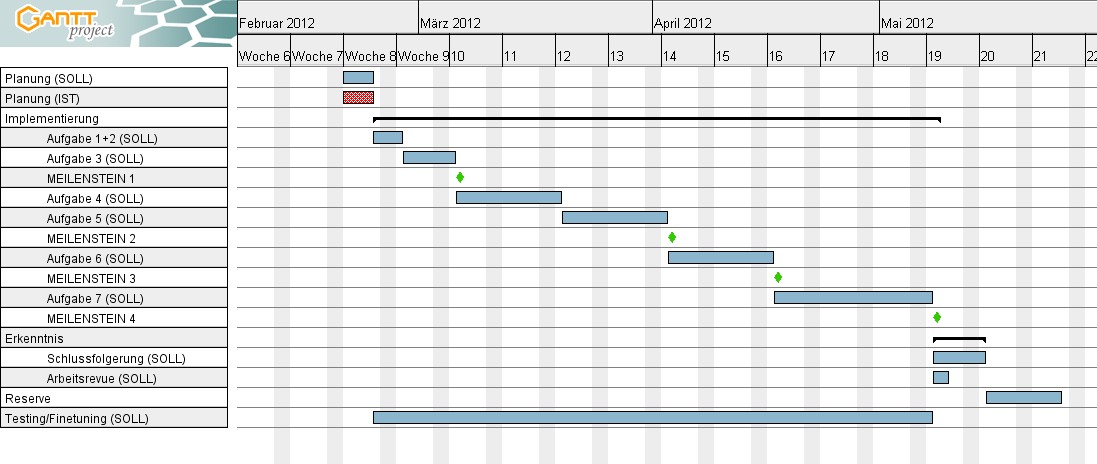
\includegraphics[width=1\linewidth]{img/projektplanung.png}
\caption{Projektplan}
\label{prplan}
\end{figure}

\subsubsection{Arbeitspakete}
Im Folgenden wird das Projekt in Arbeitspakete und ihre Abhängigkeiten eingeteilt, wie es auch in der Tabelle \ref{EffektivPlan} ersichtlich ist. Die Pakete wurden so gewählt, dass sie genau eine geschlossene Aufgabenstellung beschreiben und die Abhängigkeiten definieren, welche Arbeitspakete abgeschlossen sein müssen, damit ein bestimmtes Arbeitspaket begonnen werden kann. Desweiteren wurden auch die geplanten Dauer der Arbeitspakete angegeben. \\

Es ist festgelegt, dass beide Projektmitglieder auch gleichzeitig die
Projektleiter für die gesamte Projektlaufzeit sind. Es wird aber im
Verlauf des Projektes in jeder einzelnen Phase jeweils ein
Projektmitglied die eigentliche Projektleitung übernehmen.

Der Projektleiter der jeweiligen Phase ist hauptverantwortlich für die
rechtzeitige Fertigstellung und die Qualität des Produkts der jeweiligen
Phase.

\begin{table}[h!]
\centering 
  \begin{tabularx}{\textwidth}{| l | X | l| X | }
    \hline
    \cellcolor{hellgrau}\textbf{Nummer} & \multicolumn{3}{l |}{1}  \\ \hline
    \cellcolor{hellgrau}\textbf{Bezeichnung} & \multicolumn{3}{l |}{Aufgabe 1 \& 2} \\ \hline       
    \cellcolor{hellgrau} & \multicolumn{3}{l |}{•	Erstellung eines Entscheidungsnetzes auf der Erdkugel}  \\ 
    \cellcolor{hellgrau} & \multicolumn{3}{l |}{•	Berechnung einer Orthodromie} \\ 
    \cellcolor{hellgrau} & \multicolumn{3}{l |}{(Distanz in Meilen zwischen zwei Punkten auf der Erdkugel)}  \\ 
    \cellcolor{hellgrau} & \multicolumn{3}{l |}{•	Erstellung der Koordinatendatei eines Sees (in Koordinaten)}  \\ \cline{2-4}
    \cellcolor{hellgrau} & \multicolumn{3}{l |}{•	Erstellung eines Entscheidungskernes in dynamische Programmierung}  \\ 
     \multirow{-6}{*}{\textbf{\cellcolor{hellgrau}Beschreibung}} & \multicolumn{3}{l |}{•	Berechnung von Orthodromien auf der Erdoberfläche mit Testdaten} \\ \hline
    \cellcolor{hellgrau}\textbf{Start} & 24.02.2012 &  \cellcolor{hellgrau}\textbf{Ende} & 06.03.2012\\ \hline
    \cellcolor{hellgrau}\textbf{Abhängigkeiten} & Keine&  \cellcolor{hellgrau}\textbf{Verantwortung} & Fevzi Yükseldi\\ \hline
  \end{tabularx}
  \caption{Arbeitspaket 1}
\end{table}

\begin{table}[h!]
\centering 
  \begin{tabularx}{\textwidth}{| l | X | l| X | }
    \hline
    \cellcolor{hellgrau}\textbf{Nummer} & \multicolumn{3}{l |}{2}  \\ \hline
    \cellcolor{hellgrau}\textbf{Bezeichnung} & \multicolumn{3}{l |}{Aufgabe 3} \\ \hline       
    \cellcolor{hellgrau} & \multicolumn{3}{l |}{•	Erfassung des Polardiagramms eines Segelschiffes}  \\ 
    \cellcolor{hellgrau} & \multicolumn{3}{l |}{•	Interpolationsverfahren} \\ 
     \multirow{-3}{*}{\textbf{\cellcolor{hellgrau}Beschreibung}} & \multicolumn{3}{l |}{•	Test: Schiffgeschwindigkeiten berechnen} \\ \hline
    \cellcolor{hellgrau}\textbf{Start} & 06.03.2012 &  \cellcolor{hellgrau}\textbf{Ende} & 13.03.2012\\ \hline
    \cellcolor{hellgrau}\textbf{Abhängigkeiten} & Keine&  \cellcolor{hellgrau}\textbf{Verantwortung} & Mathias Hablützel\\ \hline
  \end{tabularx}
  \caption{Arbeitspaket 2}
\end{table}

\begin{table}[h!]
\centering 
  \begin{tabularx}{\textwidth}{| l | X | l| X | }
    \hline
    \cellcolor{hellgrau}\textbf{Nummer} & \multicolumn{3}{l |}{3}  \\ \hline
    \cellcolor{hellgrau}\textbf{Bezeichnung} & \multicolumn{3}{l |}{Aufgabe 4} \\ \hline       
    \cellcolor{hellgrau} & \multicolumn{3}{l |}{•	Erfassung des Windfeldes. Quelle: stündliche Vorhersagedaten des COSMO-2 Modells}  \\ 
    \cellcolor{hellgrau} & \multicolumn{3}{l |}{•	Interpolation auf das Entscheidungsnetzes (zwei mögliche Methoden)} \\ 
     \multirow{-3}{*}{\textbf{\cellcolor{hellgrau}Beschreibung}} & \multicolumn{3}{l |}{•	Test: Darstellung des Windfeldes auf dem Entscheidungsnetz für eine Vorhersagefrist.} \\ \hline
    \cellcolor{hellgrau}\textbf{Start} & 13.03.2012 &  \cellcolor{hellgrau}\textbf{Ende} & 20.03.2012\\ \hline
    \cellcolor{hellgrau}\textbf{Abhängigkeiten} & Keine&  \cellcolor{hellgrau}\textbf{Verantwortung} & Mathias Hablützel \\ \hline
  \end{tabularx}
  \caption{Arbeitspaket 3}
\end{table}

\begin{table}[h!]
\centering 
  \begin{tabularx}{\textwidth}{| l | X | l| X | }
    \hline
    \cellcolor{hellgrau}\textbf{Nummer} & \multicolumn{3}{l |}{4}  \\ \hline
    \cellcolor{hellgrau}\textbf{Bezeichnung} & \multicolumn{3}{l |}{Aufgabe 5} \\ \hline       
    \cellcolor{hellgrau} & \multicolumn{3}{l |}{•	Wechselwirkung Windfeld – Segelschiff}  \\ 
    \cellcolor{hellgrau} & \multicolumn{3}{l |}{•	Geometrie um das Schiff, Ableitung dessen Geschwindigkeit} \\ 
     \multirow{-3}{*}{\textbf{\cellcolor{hellgrau}Beschreibung}} & \multicolumn{3}{l |}{•	Test: Berechnung der Schiffgeschwindigkeit im Windfeld} \\ \hline
    \cellcolor{hellgrau}\textbf{Start} & 20.03.2012 &  \cellcolor{hellgrau}\textbf{Ende} & 03.04.2012\\ \hline
    \cellcolor{hellgrau}\textbf{Abhängigkeiten} & Arbeitspakete 2 \& 3 &  \cellcolor{hellgrau}\textbf{Verantwortung} & Fevzi Yükseldi\\ \hline
  \end{tabularx}
  \caption{Arbeitspaket 4}
\end{table}

\begin{table}[h!]
\centering 
  \begin{tabularx}{\textwidth}{| l | X | l| X | }
    \hline
    \cellcolor{hellgrau}\textbf{Nummer} & \multicolumn{3}{l |}{5}  \\ \hline
    \cellcolor{hellgrau}\textbf{Bezeichnung} & \multicolumn{3}{l |}{Aufgabe 6} \\ \hline       
    \cellcolor{hellgrau} & \multicolumn{3}{l |}{•	Erweiterung des geometrischen Entscheidungskerns}  \\ 
    \cellcolor{hellgrau} & \multicolumn{3}{l |}{~~~~~o	Zeitmanagement} \\ 
    \cellcolor{hellgrau} & \multicolumn{3}{l |}{~~~~~o	Rekursion} \\ 
     \multirow{-4}{*}{\textbf{\cellcolor{hellgrau}Beschreibung}} & \multicolumn{3}{l |}{•	Erstellung eines Entscheidungsbaums und Test} \\ \hline
    \cellcolor{hellgrau}\textbf{Start} & 03.04.2012 &  \cellcolor{hellgrau}\textbf{Ende} & 17.04.2012\\ \hline
    \cellcolor{hellgrau}\textbf{Abhängigkeiten} & Arbeitspakete 1 \& 4 &  \cellcolor{hellgrau}\textbf{Verantwortung} & Fevzi Yükseldi\\ \hline
  \end{tabularx}
  \caption{Arbeitspaket 5}
\end{table}

\begin{table}[h!]
\centering 
  \begin{tabularx}{\textwidth}{| l | X | l| X | }
    \hline
    \cellcolor{hellgrau}\textbf{Nummer} & \multicolumn{3}{l |}{6}  \\ \hline
    \cellcolor{hellgrau}\textbf{Bezeichnung} & \multicolumn{3}{l |}{Aufgabe 7} \\ \hline       
    \cellcolor{hellgrau} & \multicolumn{3}{l |}{•	Im Entscheidungsbaum Rückberechnung der optimalen Route}  \\ 
    \cellcolor{hellgrau} & \multicolumn{3}{l |}{•	Erstellung eines Logbuchs} \\ 
     \multirow{-3}{*}{\textbf{\cellcolor{hellgrau}Beschreibung}} & \multicolumn{3}{l |}{•	Graphische Darstellung  See, Windfeld, Entscheidungsbaum, optimale Route} \\ \hline
    \cellcolor{hellgrau}\textbf{Start} & 17.04.2012 &  \cellcolor{hellgrau}\textbf{Ende} & 08.05.2012\\ \hline
    \cellcolor{hellgrau}\textbf{Abhängigkeiten} & Arbeitspakete 1 \& 3 \& 5 &  \cellcolor{hellgrau}\textbf{Verantwortung} & \\ \hline
  \end{tabularx}
  \caption{Arbeitspaket 6}
\end{table}

\begin{table}[h!]
\centering 
  \begin{tabularx}{\textwidth}{| l | X | l| X | }
    \hline
    \cellcolor{hellgrau}\textbf{Nummer} & \multicolumn{3}{l |}{7}  \\ \hline
    \cellcolor{hellgrau}\textbf{Bezeichnung} & \multicolumn{3}{l |}{Testing / Finetuning} \\ \hline       
    \cellcolor{hellgrau} & \multicolumn{3}{l |}{•	Die Tests werden laufend durchgeführt.}  \\ 
     \multirow{-2}{*}{\textbf{\cellcolor{hellgrau}Beschreibung}} & \multicolumn{3}{l |}{•	Am Ende jedes Pakets wird die Arbeit mit realen Daten getestet} \\ \hline
    \cellcolor{hellgrau}\textbf{Start} & 24.02.2012 &  \cellcolor{hellgrau}\textbf{Ende} & 08.05.2012\\ \hline
    \cellcolor{hellgrau}\textbf{Abhängigkeiten} & Keine &  \cellcolor{hellgrau}\textbf{Verantwortung} & Alle \\ \hline
  \end{tabularx}
  \caption{Arbeitspaket 7}
\end{table}

\begin{table}[h!]
\centering 
  \begin{tabularx}{\textwidth}{| l | X | l| X | }
    \hline
    \cellcolor{hellgrau}\textbf{Nummer} & \multicolumn{3}{l |}{8}  \\ \hline
    \cellcolor{hellgrau}\textbf{Bezeichnung} & \multicolumn{3}{l |}{Bericht} \\ \hline       
    \cellcolor{hellgrau} & \multicolumn{3}{l |}{•	Einleitung.}  \\ 
    \cellcolor{hellgrau} & \multicolumn{3}{l |}{•	Vorgehen / Methoden.}  \\ 
    \cellcolor{hellgrau} & \multicolumn{3}{l |}{•	Resultate.}  \\ 
     \multirow{-4}{*}{\textbf{\cellcolor{hellgrau}Beschreibung}} & \multicolumn{3}{l |}{•	Diskussion und Ausblick} \\ \hline
    \cellcolor{hellgrau}\textbf{Start} & 24.02.2012 &  \cellcolor{hellgrau}\textbf{Ende} & 08.06.2012\\ \hline
    \cellcolor{hellgrau}\textbf{Abhängigkeiten} & Keine &  \cellcolor{hellgrau}\textbf{Verantwortung} & Alle \\ \hline
  \end{tabularx}
  \caption{Arbeitspaket 8}
\end{table}
\section{Offizielle Aufgabenstellung}

\section{Besprechungsprotokolle}


\bibliographystyle{ba_zhaw}
\bibliography{hablumat_biblio,yuksefev_biblio}
 \end{document}
